% Options for packages loaded elsewhere
\PassOptionsToPackage{unicode}{hyperref}
\PassOptionsToPackage{hyphens}{url}
%
\documentclass[
]{article}
\title{Impact of cropping system diversification on vegetative and reproductive characteristics of waterhemp (\emph{Amaranthus tuberculatus})}
\author{}
\date{\vspace{-2.5em}}

\usepackage{amsmath,amssymb}
\usepackage{lmodern}
\usepackage{iftex}
\ifPDFTeX
  \usepackage[T1]{fontenc}
  \usepackage[utf8]{inputenc}
  \usepackage{textcomp} % provide euro and other symbols
\else % if luatex or xetex
  \usepackage{unicode-math}
  \defaultfontfeatures{Scale=MatchLowercase}
  \defaultfontfeatures[\rmfamily]{Ligatures=TeX,Scale=1}
\fi
% Use upquote if available, for straight quotes in verbatim environments
\IfFileExists{upquote.sty}{\usepackage{upquote}}{}
\IfFileExists{microtype.sty}{% use microtype if available
  \usepackage[]{microtype}
  \UseMicrotypeSet[protrusion]{basicmath} % disable protrusion for tt fonts
}{}
\makeatletter
\@ifundefined{KOMAClassName}{% if non-KOMA class
  \IfFileExists{parskip.sty}{%
    \usepackage{parskip}
  }{% else
    \setlength{\parindent}{0pt}
    \setlength{\parskip}{6pt plus 2pt minus 1pt}}
}{% if KOMA class
  \KOMAoptions{parskip=half}}
\makeatother
\usepackage{xcolor}
\IfFileExists{xurl.sty}{\usepackage{xurl}}{} % add URL line breaks if available
\IfFileExists{bookmark.sty}{\usepackage{bookmark}}{\usepackage{hyperref}}
\hypersetup{
  pdftitle={Impact of cropping system diversification on vegetative and reproductive characteristics of waterhemp (Amaranthus tuberculatus)},
  hidelinks,
  pdfcreator={LaTeX via pandoc}}
\urlstyle{same} % disable monospaced font for URLs
\usepackage[margin=1in]{geometry}
\usepackage{longtable,booktabs,array}
\usepackage{calc} % for calculating minipage widths
% Correct order of tables after \paragraph or \subparagraph
\usepackage{etoolbox}
\makeatletter
\patchcmd\longtable{\par}{\if@noskipsec\mbox{}\fi\par}{}{}
\makeatother
% Allow footnotes in longtable head/foot
\IfFileExists{footnotehyper.sty}{\usepackage{footnotehyper}}{\usepackage{footnote}}
\makesavenoteenv{longtable}
\usepackage{graphicx}
\makeatletter
\def\maxwidth{\ifdim\Gin@nat@width>\linewidth\linewidth\else\Gin@nat@width\fi}
\def\maxheight{\ifdim\Gin@nat@height>\textheight\textheight\else\Gin@nat@height\fi}
\makeatother
% Scale images if necessary, so that they will not overflow the page
% margins by default, and it is still possible to overwrite the defaults
% using explicit options in \includegraphics[width, height, ...]{}
\setkeys{Gin}{width=\maxwidth,height=\maxheight,keepaspectratio}
% Set default figure placement to htbp
\makeatletter
\def\fps@figure{htbp}
\makeatother
\setlength{\emergencystretch}{3em} % prevent overfull lines
\providecommand{\tightlist}{%
  \setlength{\itemsep}{0pt}\setlength{\parskip}{0pt}}
\setcounter{secnumdepth}{-\maxdimen} % remove section numbering
\usepackage{lineno}
\linenumbers
\usepackage{float}
\usepackage{booktabs}
\usepackage{longtable}
\usepackage{array}
\usepackage{multirow}
\usepackage{wrapfig}
\usepackage{colortbl}
\usepackage{pdflscape}
\usepackage{tabu}
\usepackage{threeparttable}
\usepackage{threeparttablex}
\usepackage[normalem]{ulem}
\usepackage{makecell}
\usepackage{xcolor}
\ifLuaTeX
  \usepackage{selnolig}  % disable illegal ligatures
\fi
\usepackage[round]{natbib}
\bibliographystyle{plainnat}

\begin{document}
\maketitle

\emph{This script demonstrates how the sections were put together before final processing with Overleaf. Some typos and raw LaTeX codes may present.}

\hypertarget{abstract}{%
\section*{Abstract}\label{abstract}}
\addcontentsline{toc}{section}{Abstract}

Corn- and soybean-dominated cropping systems create and maintain a favorable environment for summer annual weeds whose emergence and growth phenology are similar to these annual summer crops. Cropping system diversification can be an effective approach for controlling noxious weeds without increasing reliance on chemical herbicides. Diversification may be especially important for managing waterhemp, a dioecious, summer annual weed that is becoming increasingly prevalent in the US Corn Belt due to its life history characteristics and herbicide resistance profile.

Compared to corn and soybean, alfalfa and oat emerge and establish earlier and are thus more competitive with warm-season weeds like waterhemp. Knowledge of vegetative and reproductive characteristics in a range of crop environments can be valuable for planning weed management strategies. However, most of the relevant characteristics for a population dynamics model were available in corn and soybean monocultures. We examined the relationship between waterhemp's aboveground mass and fecundity under four crop species' presence within three crop rotation systems: a 2-year sequence of corn and soybean; a 3-year sequence of corn, soybean, and oat intercropped with red clover; and a 4-year sequence of corn, soybean, oat intercropped with alfalfa, and alfalfa. All the rotation systems were treated with conventional or reduced rates of herbicides. We established eighteen linear equations to predict waterhemp's fecundity from dried aboveground mass in each crop and associated crop management program since measuring the latter allows for quicker estimation of fecundity compared to counting seeds on each individual plant.

Rotation system and crop phase within rotation system had significant effects on all the response variables but weed control regime on some. The sex ratios at maturity were slightly female-biased in oat and alfalfa. Mature female plants were generally larger than male. Mature waterhemp plants were larger in corn and soybean than in oat and alfalfa. Oat and alfalfa were planted earlier than corn and soybean and successfully competed for resources against waterhemp despite the absence of herbicide or interrow cultivation. Frequent hay cuts in alfalfa served as physical weed control and contributed to suppressing waterhemp and other weeds substantially.

\hypertarget{introduction}{%
\section*{Introduction}\label{introduction}}
\addcontentsline{toc}{section}{Introduction}

Cropping system diversification can contribute to the effective suppression of noxious weeds such as velvetleaf (\emph{Abutilon theophrasti} Medik.) \citep{westermanAreManyLittle2005}, giant foxtail (\emph{Setaria faberi} Herrm.) \citep{liebmanFatesSetariaFaberi2014}, giant ragweed (\emph{Ambrosia trifida} L.) \citep{liebmanCroppingSystemRedesign2020}, and other species while complementing the effects of herbicides and physical weed control practices \citep{davisIncreasingCroppingSystem2012, weisbergerDoesDiversifyingCrop2019}.
Much of the effectiveness of diversified cropping systems for weed suppression can be attributed to differences among crop species in their phenologies and the management techniques applied to them. Differences in crop phenology and diverse management tactics can lead to a net loss in weed seed population density in the soil seed bank \citep{maclarenEcologicalFutureWeed2020, liebmanManyLittleHammers1997} resulting from reductions in weed fecundity and increased consumption of weed seeds by granivores. The present study focuses on fecundity and other relevant individual- and population-level reproductive and vegetative characteristics of waterhemp (\emph{Amaranthus tuberculatus} (Moq.) J. D. Sauer) in three rain-fed cropping systems differing in crop species richness and management practices.

Waterhemp is a dioecious, summer annual, dicotyledonous species that has been listed as one of the five most noxious weeds in row crops in the U.S. based on the number of times this species appears in the literature \citep{johnsonInfluenceGlyphosateresistantCropping2009} and by growers' concern across 22 states in the U.S. \citep{princeBenchmarkStudyIV2012}. At least 54 waterhemp populations are resistant to up to five herbicide modes of action as of 2021 \citep{heapHerbicideResistantTall2021}.

As a dioecious species, populations of waterhemp are expected to express a 1:1 male:female ratio \citep{grantCytogeneticStudiesAmaranthus1959, costeaBiologyInvasiveAlien2005, heneghanGrowthDevelopmentFive2017}. However, waterhemp has three characteristics that favor female-biasedness under conditions of no stress, according to a study of 243 dioecious species excluding waterhemp \citep{fieldComparativeAnalysesSexratio2013}: 1) the male sex is heterogametic \citep{montgomeryMaleSpecificChromosomal2021}; 2) the species has abiotic pollination and seed dispersal; and 3) the fruits are non-fleshy \citep{costeaBiologyInvasiveAlien2005}. A stressed waterhemp population tends to be female-biased, with up to ten females per male \citep{prattAmaranthusRudisTuberculatus2001}, which is consistent with the general pattern of sexually differentiated stress tolerance in herbaceous plants \citep[38 species, excluding waterhemp,][]{juvanySexrelatedDifferencesStress2015}. The sex ratio plasticity of waterhemp suggests that a stressed population, which is characterized by low-density, may allocate available resources to produce more female offspring as an effort to increase population density, as observed in its close relative, Palmer amaranth (\emph{A. palmeri}) \citep{korresPalmerAmaranthAmaranthus2017, mesgaranSexLabilityDimorphism2019}. Knowing how sex ratios may deviate from parity under different biotic and abiotic conditions could inform how a waterhemp population might progress from one generation to the next.

Waterhemp management is agronomically challenging because of a suite of life history characteristics, including a persistent soil seedbank \citep{davisWeedSeedPools2008}, an extended seedling emergence pattern \citep{buhlerEmergencePersistenceSeed2001}, high relative growth rate, high fecundity \citep{heneghanGrowthDevelopmentFive2017}, and rapid herbicide resistance development \citep{tranelHerbicideResistanceAmaranthus2021}. One year of prolific seed production can replenish a declining seedbank with more seeds than existed in the seedbank \citep{davisWeedSeedPools2008}. Failing to control waterhemp can cause up to 43\% yield loss in soybean (\emph{Glycine max} (L.) Merr.) \citep{hagerCommonWaterhempAmaranthus2002a} and 74\% yield loss in corn (\emph{Zea mays} L.) \citep{steckelCommonWaterhempAmaranthus2004}.

The accumulated mass and density of a weed population reflect the relative competitiveness against crops and the favorability of the environment, which in turn could signal the effectiveness of weed management throughout the season. From a planning perspective, population density at maturity and plant fecundity are useful for estimating the density of new seeds produced and potentially added to the soil seedbank, and for adjusting weed management regimes accordingly \citep{buhlerImplicationsWeedSeedbank1997}. Waterhemp's fecundity has been studied in corn and soybean crops \citep{menalledImpactCompostedSwine2004, nordbyInfluenceCornCommon2004} but not in other crops' or in an extended crop rotation system.
Alfalfa (\emph{Medicago sativa} L.), red clover (\emph{Trifolium pratense} L.), and oat (\emph{Avena sativa} L.) are cool-season crops that can be grown in rotation sequences with corn and soybean, whereas waterhemp is a summer annual weed. Compared to corn and soybean, alfalfa, red clover, and oat seedlings emerge and establish earlier. Alfalfa, red clover, and oat also emerge and establish earlier than a number of summer annual weed species, including waterhemp \citep{buhlerRelativeEmergenceSequence2008, horakGrowthAnalysisFour2000}.

In the present study, we examined the population aboveground mass, density and sex ratio, male-female size difference, and the relationship between waterhemp's female size and fecundity when the weed grew in association with five crop species (corn, soybean, oat, red clover, and alfalfa) arranged in three rain-fed cropping systems. Assessing waterhemp characteristics in the presence of oat intercropped with red clover or alfalfa and alfalfa grown as a sole crop as well as corn and soybean could help to fill the gap of information concerning waterhemp performance in extended rotations.

We hypothesized that the sex ratio of a waterhemp population deviated from parity depending on the environment's favorability, but how much and to which direction the shift would occur would depend on how much the studied population was suppressed. In addition to informing management, individual- and population-level characteristics would provide useful contextual details for sex ratio comparison.

Counting seeds for waterhemp fecundity assessment is time-consuming and laborious, so it would be convenient to extrapolate fecundity from plant mass. We hypothesized that regression relationships with which to predict fecundity from plant mass could be identified but that such relationships would differ among treatments, due to differences in crop phenology, crop-weed competition, and management practices.

\hypertarget{materials-and-methods}{%
\section*{Materials and Methods}\label{materials-and-methods}}
\addcontentsline{toc}{section}{Materials and Methods}

\hypertarget{experiment-design}{%
\subsection*{Experiment Design}\label{experiment-design}}
\addcontentsline{toc}{subsection}{Experiment Design}

Empirical measurements of waterhemp biomass and fecundity were made in 2018 at Iowa State University's Marsden Farm in Boone County, Iowa, USA, (42\(^\circ\) 01'N, 93\(^\circ\) 47'W, 333 m above sea level). The site description and crop management practices were described by \citet{liebmanWeedSeedbankDiversity2021}.

The experiment was initiated in 2001 on a 9-hectare field to compare the performance of three different crop rotations. In 2008, the experiment was reorganized to allow comparison of two contrasting weed management regimes in each of the three rotation systems.

In the present study, the experiment comprised of 72 experimental units each 9 m x 84 m. The experimental units (eu) were arranged in a randomized complete block split-plot design with four replications. The experiment was two-way factorial, with crop rotations comprising main plots and weed management regimes comprising split plots. Within each of the four blocks, plots were randomly assigned to one of the crop phases within one of three rotations. In any year, all crop phases within the same rotation were present in different plots in the same replicate block to avoid confounding effects of the year with those of the treatments \citep{payneDesignAnalysisLong2015}. The 2-year, 3-year, and 4-year crop sequences included in the study are shown in Table \ref{tab:sequence}. The conceptual diagram for the experiment is shown in Figure \ref{fig:concept}.

Alfalfa in this experiment was sown with oat. Oat was harvested for grain in 2018 and for hay in 2019 and alfalfa was retained over the winter and used as a hay crop the following year. Oat in our experiment was intended for grain harvest but was harvested for hay in 2019 due to high weed infestation and hailstorm damage at oat's critical stage. In the conventional weed management regime, herbicide was broadcast on the whole area that was planted to corn, whereas in the low herbicide regime, herbicide was applied in 38-cm bands over corn rows, and interrow areas were cultivated. Even though corn was the only crop that received the contrasting weed management regimes, all other crops were identified with the weed management applied to the corn phase (hereafter referred to as \emph{corn weed management}), to which they followed. To improve weed control efficacy, herbicides used for soybean differed between 2018 and 2019. Details concerning crop genotypes and management practices are shown in Table \ref{tab:crop-id}.

\begin{landscape}\begin{table}

\caption{\label{tab:crop-id}Crop varieties, and dates and rates for management operations in 2018 and 2019. Oat and red clover were intercropped in the 3-year system. Oat and alfalfa were intercropped in the third year of the 4-year system and alfalfa was overwintered after oat harvest.}
\centering
\fontsize{8}{10}\selectfont
\begin{tabular}[t]{>{\raggedright\arraybackslash}p{4em}l>{\raggedright\arraybackslash}p{6em}>{\raggedright\arraybackslash}p{6em}>{\raggedright\arraybackslash}p{8em}>{\raggedright\arraybackslash}p{5em}>{\raggedright\arraybackslash}p{8em}>{\raggedright\arraybackslash}p{5em}>{\raggedright\arraybackslash}p{5em}>{\raggedright\arraybackslash}p{15em}}
\toprule
Rotation & Crop & Hybrid or cultivar & Planting date & Harvest date & Seed density & Crop density & Interrow & Cultivation & Herbicide (kg ai/ha)\\
\midrule
\addlinespace[0.3em]
\multicolumn{10}{l}{\textbf{2018 season}}\\
\hspace{1em} &  &  &  &  & seedsm\$\textasciicircum{}\{-2\}\$ & plantsm\$\textasciicircum{}\{-2\}\$ & cm &  \vphantom{1} & \\
all & corn & Epley 1420 & May. 8 & Oct. 30 & 8 & 8 & 76 & low: Jun. 4; conv: none & low: tembotrione (0.054); conv: PRE thiencarbazone methyl (0.037), isoxaflutole (0.093); POST: mesotrione (0.105), nicosulfuron (0.053)\\
all & soybean & Latham 2758 R2 & Jun. 3 & Oct. 29 & 35 & 18 & 76 & none & flumioxazin (0.096); POST: glyphosate as potassium salt (1.540), lactofen (0.140)\\
 &  &  &  &  & kgm\$\textasciicircum{}\{-2\}\$ &  & cm &  & \\
3- and 4-year & oat & INO9201 & Apr. 24 & Jul. 20 & 0.009 & 225 (3-year) and 236 (4-year) & 20 & none & none\\
3-year & red clover & Mammoth Red & Apr. 24 &  & 0.002 & 187 & 20 & none & none\\
4-year & alfalfa & 55H94 & Apr. 12, 2017 & Jun. 4, Jul. 9, and Sep. 10 & 0.002 & 154 & 20 & none & none\\
\addlinespace[0.3em]
\multicolumn{10}{l}{\textbf{2019 season}}\\
\hspace{1em} &  &  &  &  & seedsm\$\textasciicircum{}\{-2\}\$ & plantsm\$\textasciicircum{}\{-2\}\$ & cm &  & \\
all & corn & Epley 1730 & Jun. 3 & Nov. 6 & 8 & 8 & 76 & none & low: tembotrione (0.0054); conv: PRE: thiencarbazone methyl (0.037), isoxaflutole (0.093); POST: mesotrione (0.105), nicosulfuron (0.053)\\
all & soybean & Latham 2758 R2 & Jun. 10 & Oct. 18 & 35 & 31 & 76 & none & PRE: flumioxazin (0.096); POST: glufosinate ammonium (0.594), clethodim (0.136)\\
 &  &  &  &  & kgm\$\textasciicircum{}\{-2\}\$ &  & cm & none & none\\
3- and 4-year & oat & INO9201 & Apr. 16 & Jul. 22 and 24 & 0.009 & 366 (3-year) and 330 (4-year) & 20 & none & none\\
3-year & red clover & Mammoth & Apr. 16 &  & 0.002 & 219 & 20 & none & none\\
4-year & alfalfa & WS Leafguard & Apr. 24 & Jun. 7, Jul. 12, Aug. 26, & 0.002 & 176 & 20 & none & none\\
\bottomrule
\end{tabular}
\end{table}
\end{landscape}

\begin{table}

\caption{\label{tab:sequence}Crop phases of the three rotation systems present in a replicate block in 2018 and 2019}
\centering
\begin{tabular}[t]{l|c|c|c|c|c|c|c|c|c}
\hline
 & 2-year & 2-year & 3-year & 3-year & 3-year & 4-year & 4-year & 4-year & 4-year\\
\hline
2018 & corn & soybean & corn & soybean & oat/red clover & corn & soybean & oat/alfalfa & alfalfa\\
2019 & soybean & corn & soybean & oat/red clover & corn & soybean & oat/alfalfa & alfalfa & corn\\
\hline
\end{tabular}
\end{table}

\textbackslash begin\{figure\}{[}H{]}
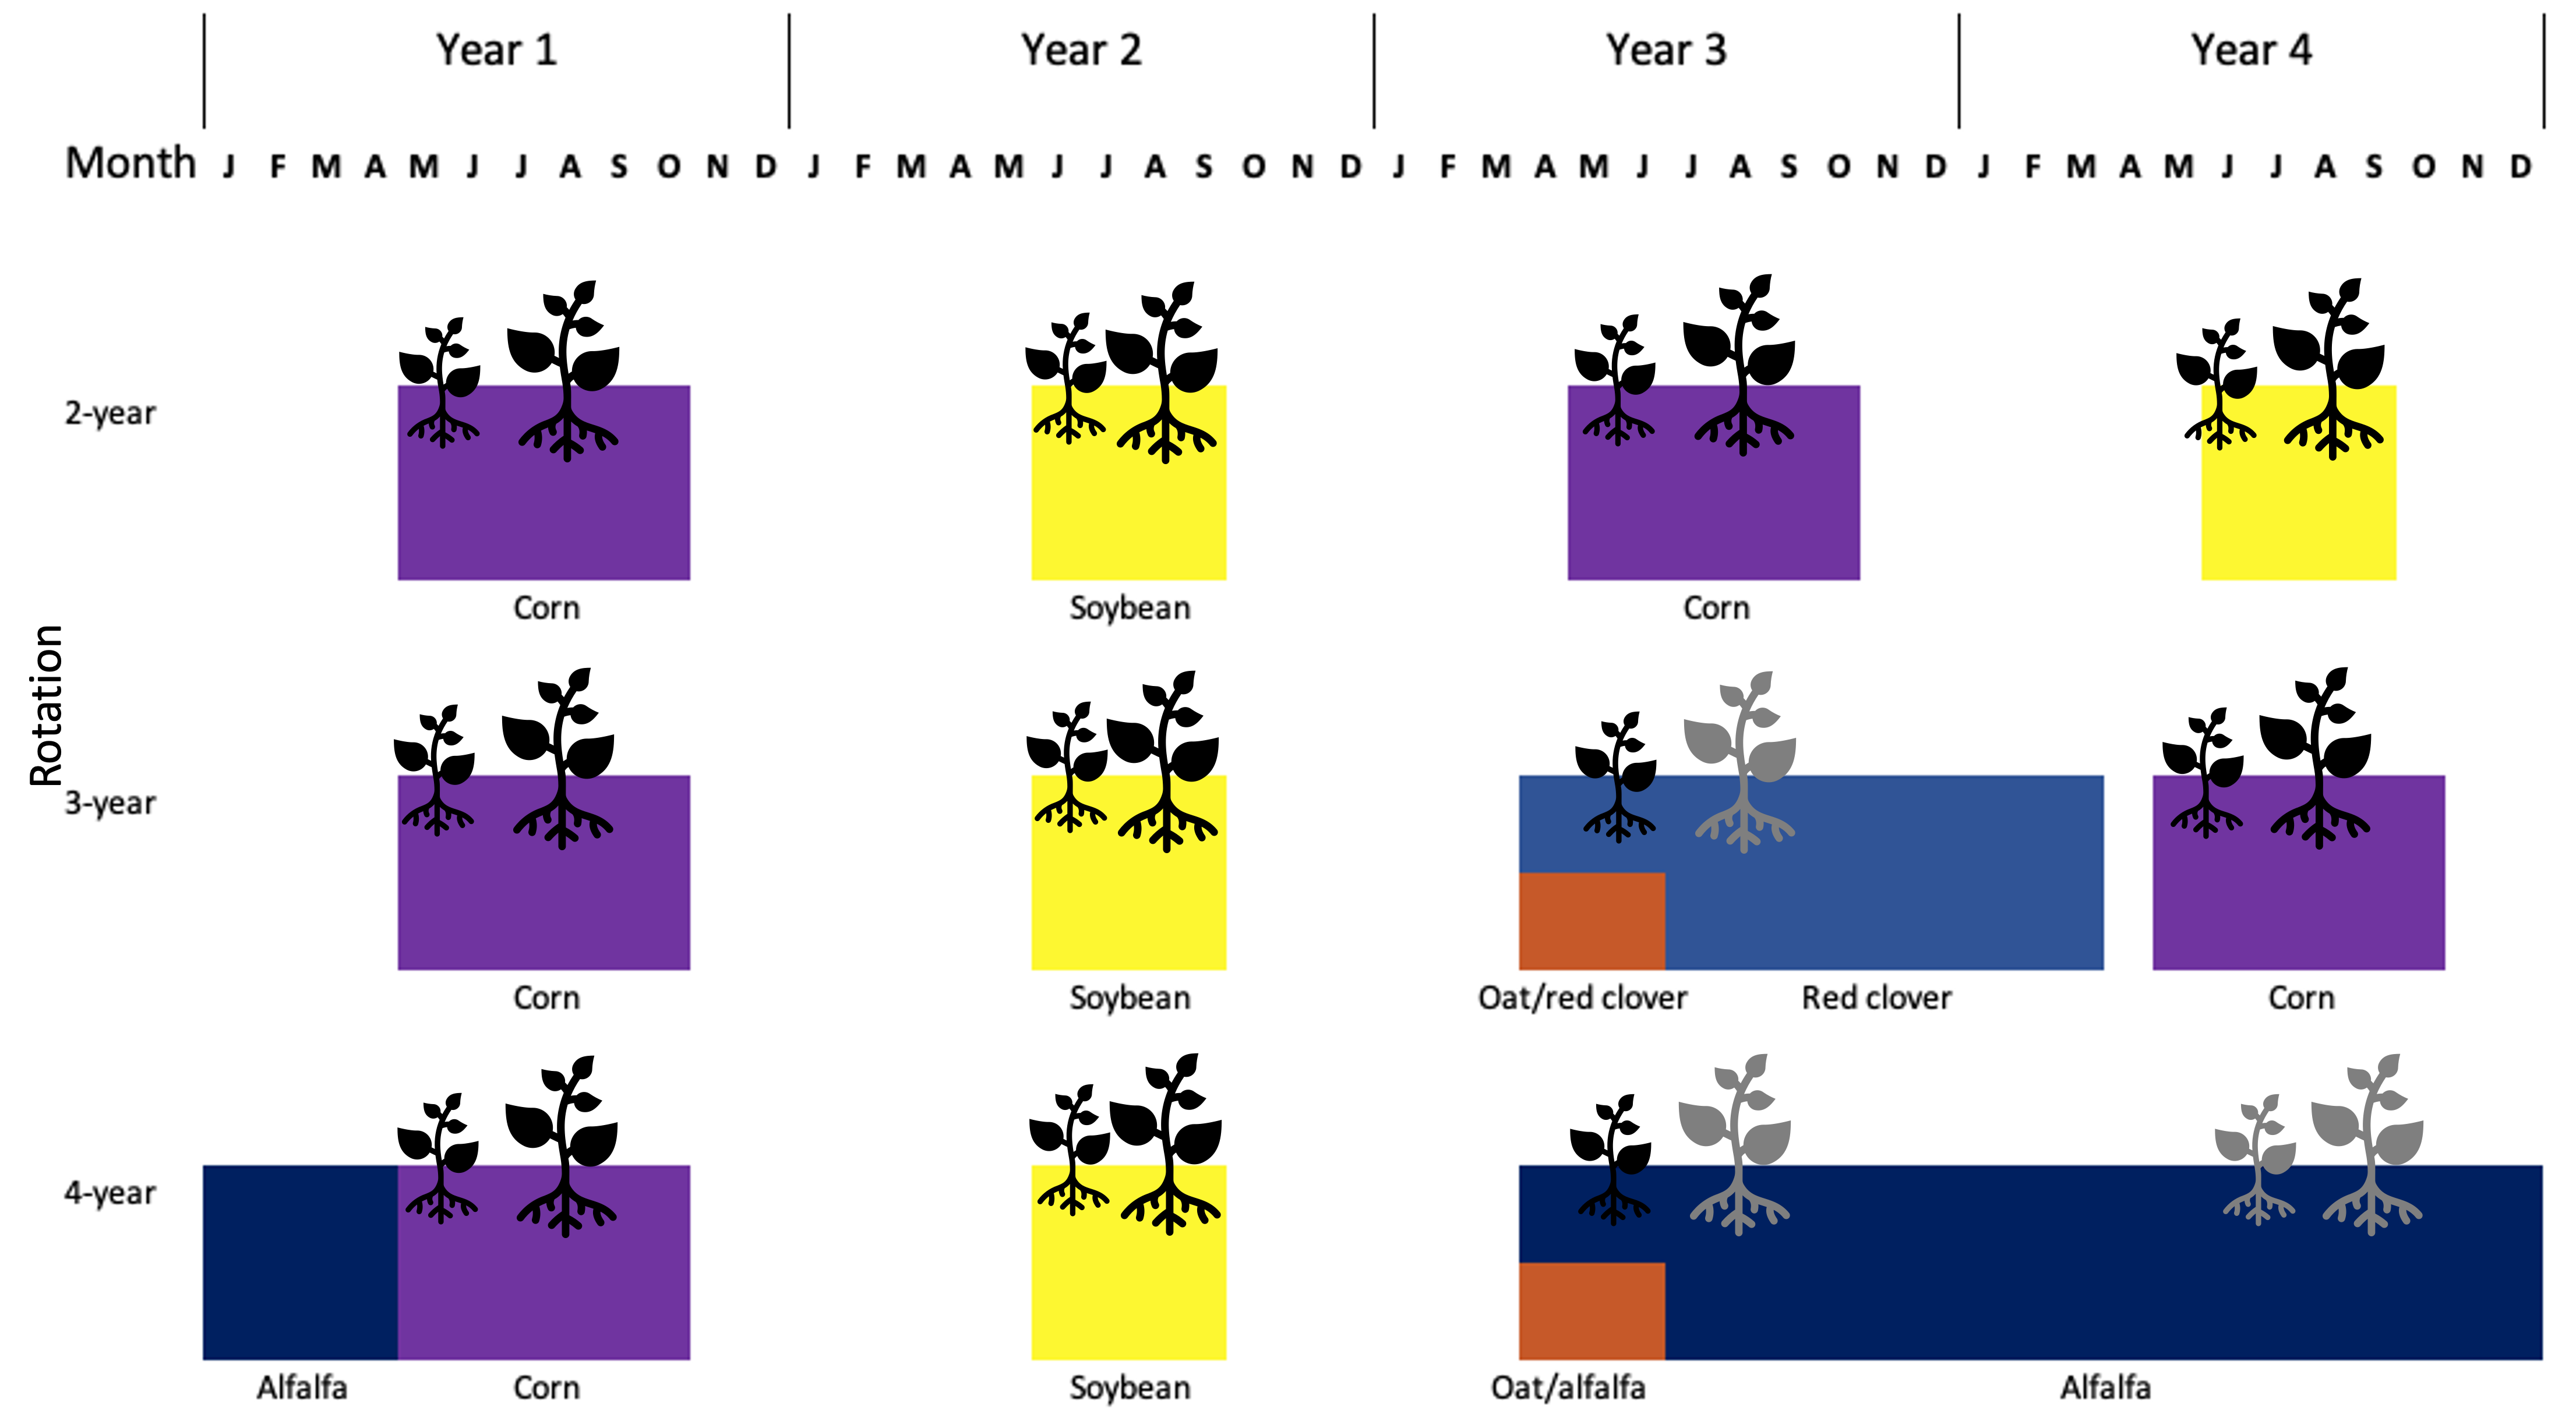
\includegraphics[width=1\linewidth]{concept} \textbackslash caption\{Conceptual diagram of the three rotation systems compared within the experiment. A cycle of four calendar years is shown. Crops are color-coded and displayed for the approximate months that they were present. Emergence and establishment of common waterhemp plants are illustrated with black symbols. Grey plants shown in oat or alfalfa's first year were physically controlled by crop harvest operations. Grey plants shown in alfalfa's second year were physically suppressed three to four times by haynharvest. Alfalfa's hay was harvested when approximately 5\% of the plants flowered.\}\label{fig:concept}
\textbackslash end\{figure\}

\hypertarget{sample-collection}{%
\subsection*{Sample collection}\label{sample-collection}}
\addcontentsline{toc}{subsection}{Sample collection}

Samples for all response variables were collected at least 3m in from the border of each eu to avoid the possible edge effects.
For each response variable, samples were collected from eight quadrats per eu to account for the patchiness of the weed populations. In 2018, the sex ratio was assessed by scouting the whole eu to obtain higher degrees of freedom.
The date of sample collection and total sampled area for population- and individual-based measurements are shown in Table \ref{tab:sample-id}.

\begin{landscape}\begin{table}

\caption{\label{tab:sample-id}Sampling dates and areas in 2018 and 2019}
\centering
\fontsize{8}{10}\selectfont
\begin{tabular}[t]{llllll}
\toprule
\multicolumn{2}{c}{ } & \multicolumn{2}{c}{2018} & \multicolumn{2}{c}{2019} \\
\cmidrule(l{3pt}r{3pt}){3-4} \cmidrule(l{3pt}r{3pt}){5-6}
Measurement & crop & collection date & sampled area (m\textasciicircum{}2) & collection date & sampled area (m\textasciicircum{}2)\\
\midrule
Measurement & Crop & Collection date & sampled area (m\textasciicircum{}2) & Collection date & Sampled area (m\textasciicircum{}2)\\
Population above-ground mass & corn & Sep. 11, 12, 13 & 148.3 & Sep. 17, 18, 19 & 148.3\\
 & soybean & Sep. 17, 19, 21 & 148.3 & Sep. 30 & 148.3\\
 & oat & Sep. 27; Oct. 4, 15, 16, 18, 19 & 16 & Sep 23, 25, 26; Oct. 3, 4, 7 & 17.9\\
 & alfalfa & Sep. 26, 27; Oct 16, 19 & 16 & Sep 24, 25; Oct. 3, 7 & 17.9\\
Population density & corn & Sep. 11, 12, 13 & 148.3 & Sep. 17, 18, 19 & 148.3\\
 & soybean & Sep. 17, 19, 21 & 148.3 & Sep. 30 & 148.3\\
 & oat & Sep. 27; Oct. 4, 15, 16, 18, 19 & 16 & Sep 23, 25, 26; Oct. 3, 4, 7 & 17.9\\
 & alfalfa & Sep. 26, 27; Oct 16, 19 & 16 & Sep 24, 25; Oct. 3, 7 & 17.9\\
Population sex ratio & corn & Sep. 10, 11, and 12 & 729 & Sep. 17, 18, and 19 & 148.3\\
 & soybean & Sep. 17 and 30 & 729 & Sep. 30 & 148.3\\
 & oat & Oct. 4, 15, and 18 & 729 & Sep. 24, 25, 26, 30, Oct. 1 and 2 & 17.9\\
 & alfalfa & Nov. 1 & 729 & Oct. 3 and 4 & 17.9\\
Individual female above-ground mass & corn & Oct. 18, 19, 22,  24, and 25 & 729 & Sep. 17, 18, and 19 & 148.3\\
 & soybean & Oct. 4, 15, and 18 & 729 & Sep. 30 & 148.3\\
 & oat & Oct. 29, 30, 31, Nov. 1 & 729 & Sep. 24, 25, 26, 30, Oct. 1 and 2 & 17.9\\
 & alfalfa & Nov. 1 & 729 & Oct. 3 and 4 & 17.9\\
Individual female fecundity & corn & Oct. 24 and 25 & 729 & none & none\\
 & soybean & Oct. 4, 15, and 18 & 729 & none & none\\
 & oat & Oct. 29, 30, 31, Nov. 1 & 729 & none & none\\
 & alfalfa & Nov. 1 & 729 & none & none\\
\bottomrule
\end{tabular}
\end{table}
\end{landscape}

\hypertarget{population-sex-ratio}{%
\subsubsection*{Population sex ratio}\label{population-sex-ratio}}
\addcontentsline{toc}{subsubsection}{Population sex ratio}

In 2018 we scouted each eu until 100 or all the available plants (if the number of plants available was fewer than 100) were sexed to obtain greater degrees of freedom. We determined the sex of 252, 1999, 2426, and 895 waterhemp plants in alfalfa, oat, soybean, and corn, respectively. In 2019, eight quadrats per eu were marked at the beginning of the season and fixed until crop harvest for a census. Overall, 413, 1331, 0, and 553 waterhemp plants were sexed in alfalfa, oat, soybean, and corn, respectively. Zero observations in all the soybean eu's resulted from high herbicide efficacy, so the 2019 data was imputed (Appendix B).

\hypertarget{population-aboveground-mass-and-density}{%
\paragraph{Population aboveground mass and density}\label{population-aboveground-mass-and-density}}

The quadrats were randomly placed in a 4 x 2 grid at the sampling date and were non-overlapping with the 2019 census quadrats. The number of plants and the total dried biomass was tallied by eu.

\hypertarget{individual-female-aboveground-mass-and-fecundity}{%
\paragraph{Individual female aboveground mass and fecundity}\label{individual-female-aboveground-mass-and-fecundity}}

The maturation of waterhemp seeds can take 20 days from pollination \citep{bellTimeRequirementPollination2010}.
We harvested female waterhemp plants as close to crop harvest as possible to maximize the number of mature seeds on mother plants. Prior to sample collection in an eu, the whole area was visually inspected to estimate the difference in plant sizes. Specimens were then collected to best capture the range of within-eu variance.
Given the time and labor constraints, we planned to collect eight intact plants from each eu, which was equivalent to 576 plants in total. Plants had to be identifiable per \citet{uvaWeedsNortheast1997}. By the time the seeds reached maturity, 389 intact plants were collected and processed. No intact plants were collected from two eu's.
Plant specimens were contained individually in tightly knitted fabric bags to prevent seed loss. The detailed procedure for seed cleaning and counting is provided in Appendix A.

\hypertarget{model-fitting-and-selection}{%
\subsection*{Model fitting and selection}\label{model-fitting-and-selection}}
\addcontentsline{toc}{subsection}{Model fitting and selection}

Waterhemp survival in soybean was the greatest among all crops in the experiment in 2018 but the least in 2019 because of the use of different herbicide active ingredients. Given year-to-year differences in the sampling scheme and herbicide efficacy, the two years of data were thus analyzed separately for all the response variables in R version 4.1.2 \citep{rdevelopmentcoreteamLanguageEnvironmentStatistical2021}. The data was curated with the \texttt{tidyverse} package \citep[version 1.3.1,][]{wickhamTidyverseEasilyInstall2021}.

In 2018, 2\% of the sex ratio data was missing due to zero observations in one eu, so complete case analysis, in which eu of unknown sex ratio was removed from the data set, was used. In 2019, 22\% of the sex ratio data was missing, so the data were imputed with predictive mean matching (PMM) method with the \texttt{mice} package \citep[version 3.13.0,][]{vanbuurenMiceMultivariateImputation2011} to optimally replace missing data with meaningful values without altering the observed sex ratios (Appendix). Any model that involved the imputed data was fitted on all the produced (imputed) data sets, and the results were pooled \citep{whiteMultipleImputationUsing2011}.

Block was included in all models as a fixed factor because blocks were used to control the different field conditions across sections, and thus to reduce variance between eu's \citep{dixonShouldBlocksBe2016}. All the models were first fitted full, with block, corn weed management and crop identity, the interaction of corn weed management and crop identity, and covariates when applicable, then reduced to remove non-significant factors. Crop identity is the combination of crop species and the rotation to which they belonged. The within-eu variation was random and absorbed in the random error term in each model equation. The fitted models were linear (\texttt{lm}), generalized linear (\texttt{glm}), or generalized least square (\texttt{gls}) depending on the data structure and the nature of the response variable. The response and quantitative variables were appropriately transformed as needed to obtain homogeneous variances. Half of the minimum, non-zero value among all the observations was added to all the observations before ln-transformation to replace zeros. Response variables that were all non-zero were ln-transformed without adjustment. The goodness of fit of each model was assessed with diagnosis plots and mean squared error (MSE) of the variance.

The marginal means of each response variable were estimated with the \texttt{emmeans} function from the \texttt{emmeans} package \citep[version 1.7.1-1][]{lenthEmmeansEstimatedMarginal2021} to accommodate non-integer and unequal degrees of freedom among groups. Marginal means were averaged over blocks for post- ANOVA or ANCOVA contrasts. Degree of freedom adjustment was done with the Satterthwaite method for the \texttt{gls} and Kenward-Roger method for the \texttt{glm} and \texttt{lm} models.\\
ANCOVA (analysis of covariance) was applied to examine the effect of treatments on the relationship between female aboveground biomass and fecundity and between population sex ratio and biomass or density at maturity.
ANCOVA combines regression and ANOVA (analysis of variance) to improve precision in mean estimation as compared to ANOVA estimation \citep{yangAnalysisCovarianceAgronomy2011}.\\
Type III sums of squares error were calculated with the \texttt{emmeans}`s \texttt{joint\_tests} function to accommodate unbalanced data with interaction when occurred and to avoid misleading assessment of factors' effects based on their sequential order in the model.

\hypertarget{population-sex-ratio-at-maturity}{%
\subsubsection*{Population sex ratio at maturity}\label{population-sex-ratio-at-maturity}}
\addcontentsline{toc}{subsubsection}{Population sex ratio at maturity}

A logistic regression model was fitted with the \texttt{glm} command and \texttt{family\ =\ quasibinomial(link\ =\ logit)} argument specification to analyze sex ratio. The \texttt{quasibinomial} family with follow-up F-test was used to accommodate overdispersion and \texttt{logit} link function transformed the sex ratio using the natural logarithm (ln) \citep{crawleyProportionData2013}.

\[ S_{ijk} = Binomial\,(N_{ijk},\pi_{ijk}) \]

\begin{align}
ln \frac{\pi_{ijk}}{1-\pi_{ijk}} = \mu + b_k + \alpha_i + \gamma_j +\alpha_i \gamma_j + \epsilon_{ijk} \label{eq:sex-mature}
\end{align}

where,

\(S_{ijk}\) is the number of female plants among all the \(N_{ijk}\) plants in block \(k^{th}\) under crop identity \(i^{th}\) and corn weed management \(j^{th}\),\\
\(ln \frac{\pi_i}{1-\pi_i}\) is the logit transformation of \(S_{ijk}\),\\
\(\mu\) is the overall mean female proportion, the intercept,\\
\(\alpha_i\) is the effect of the \(i^{th}\) crop identity,\\
\(\gamma_j\) is the effect of the \(j^{th}\) corn weed management,\\
\(b_k\) is the block effect,\\
\(\alpha_i \gamma_j\) is the interaction effect of crop identity and corn weed management, and\\
\(\epsilon_{ijk}\) is the random error.

\hypertarget{population-aboveground-mass-and-density-1}{%
\subsubsection*{Population aboveground mass and density}\label{population-aboveground-mass-and-density-1}}
\addcontentsline{toc}{subsubsection}{Population aboveground mass and density}

A linear regression model was fitted with the \texttt{lm} command on each of the two variables, population aboveground mass or stand density. The general model equation for these response variables is

\begin{align}
Y_{ijk} = \mu + b_k + \alpha_i + \gamma_j +\alpha_i \gamma_j + \epsilon_{ijk} \label{eq:pop-mass-dens}
\end{align}

where,

\(Y_{ijk}\) is either the ln-transformed population aboveground mass or ln-transformed stand density in block \(k^{th}\) under crop identity \(i^{th}\) and corn weed management \(j^{th}\),\\
and other terms as defined in Equation \eqref{eq:sex-mature}.

\hypertarget{ancova-of-population-sex-ratio-aboveground-mass-and-density}{%
\subsubsection*{ANCOVA of population sex ratio, aboveground mass, and density}\label{ancova-of-population-sex-ratio-aboveground-mass-and-density}}
\addcontentsline{toc}{subsubsection}{ANCOVA of population sex ratio, aboveground mass, and density}

The regression of sex ratio against population density or biomass was extended from the ANOVA of sex ratio (Equation \eqref{eq:sex-mature}.

\[ S_{ijk} = Binomial\,(N_{ijk},\pi_{ijk}) \]

\begin{align}
ln \frac{\pi_{ijk}}{1-\pi_{ijk}} = \mu + b_k + \alpha_i + \gamma_j +\alpha_i \gamma_j + \delta D_{ijk}  + \alpha_i D_{ijk} + \gamma_j D_{ijk} + (\alpha_i \gamma_j)D_{ijk} + \epsilon_{ijk} \label{eq:sex-mature-anc}
\end{align}

where,

\(\delta\) is the effect of the covariate,\\
\(D_{ijk}\) is the natural log-transformed population stand density in block \(k^{th}\) under crop identity \(i^{th}\), and corn weed management \(j^{th}\), the covariate,\\
and other terms as defined in Equation \eqref{eq:sex-mature}.

\hypertarget{individual-female-aboveground-mass-and-fecundity-1}{%
\subsubsection*{Individual female aboveground mass and fecundity}\label{individual-female-aboveground-mass-and-fecundity-1}}
\addcontentsline{toc}{subsubsection}{Individual female aboveground mass and fecundity}

A compound symmetric linear regression model (with \texttt{nlme} package's \texttt{gls} command was first fitted for each of the response variables, individual aboveground mass and fecundity to accommodate negative variance that occurred when the within-eu variance was larger than the between-eu variance and correlated errors occurred within blocks \citep[version 3.1-153][]{pinheroNlmeLinearNonlinear2021}.
The \texttt{corCompSymm} argument in the \texttt{gls} command was specified by identifying unique combinations of block and treatment. The model in this exercise is of the same form as the model in Equation \eqref{eq:pop-mass-dens}:

\begin{align}
Y_{ijkl} = \mu + b_k + \alpha_i + \gamma_j +\alpha_i \gamma_j + \epsilon_{ijkl} \label{eq:indiv-mass-fecund}
\end{align}

where,\\
\(Y_{ijkl}\) is either the ln-transformed aboveground mass or ln-transformed number of seeds of female plant \(l^{th}\) in block \(k^{th}\) under crop identity \(i^{th}\) and corn weed management \(j^{th}\),\\
\(\epsilon_{ijkl}\) is the random error,\\
and other terms as defined in Equation \eqref{eq:sex-mature}.

\hypertarget{individual-female-aboveground-mass-and-fecundity-relationship}{%
\subsubsection*{Individual female aboveground mass and fecundity relationship}\label{individual-female-aboveground-mass-and-fecundity-relationship}}
\addcontentsline{toc}{subsubsection}{Individual female aboveground mass and fecundity relationship}

The regression of individual plant fecundity against individual plant aboveground mass was combined from the ANOVA of each (Equation \eqref{eq:indiv-mass-fecund}) to establish a relationship between the two variables:

\begin{align} 
Y_{ijkl} = \mu + b_k + \alpha_i + \gamma_j +\alpha_i \gamma_j + \beta X_{ijkl} + \alpha_i X_{ijkl} + \gamma_j X_{ijkl} + (\alpha_i \gamma_j)X_{ijkl} + \epsilon_{ijkl} \label{eq:mass-fecund-anc}
\end{align}
where,

\(Y_{ijkl}\) is the number of seeds of plant \(l^{th}\) in block \(k^{th}\) under crop identity \(i^{th}\) and corn weed management \(j^{th}\),\\
\(X_{ijkl}\) is the dried aboveground mass of plant \(l^{th}\) in block \(k^{th}\) under crop identity \(i^{th}\), and corn weed management \(j^{th}\), the covariate,\\
and other terms as defined in Equation \eqref{eq:sex-mature}.

We tested the assumption that all the regression lines were parallel. Violation of this assumption required an individual regression line for each treatment.
To test model robustness, samples in each treatment were pooled across four blocks and divided into four size-based subsets. Samples from each subset were then randomly placed into the testing and training sets using the 80 testing : 20 training ratio. A model was considered to perform well if the data points in the testing set blended well with the data points from the training set, and a relatively small MSE was obtained. A robust model could be used to predict plant fecundity with new biomass data.

\hypertarget{results}{%
\section*{Results}\label{results}}
\addcontentsline{toc}{section}{Results}

Using \texttt{ggResidpanel} version 0.3.0 for model diagnosis \citep{goodeGgResidpanelPanelsInteractive2019}, no predictable pattern in the plots of residuals versus predicted values suggests that the analysis models fit the data well (Details are provided in the Data Repository).\\
In all rotations, all the crop yields were comparable to those of Iowa and Boone County (where the experiment is situated) \citep{nguyenWeedCommunityCompositioninpreparation}.

\hypertarget{individual-female-aboveground-mass-and-fecundity-2}{%
\subsection*{Individual female aboveground mass and fecundity}\label{individual-female-aboveground-mass-and-fecundity-2}}
\addcontentsline{toc}{subsection}{Individual female aboveground mass and fecundity}

Individual female aboveground mass and fecundity were affected by rotation, crop species, and corn weed management (Table \ref{tab:f-biom-fecund-ct}). Crop identity was more influential on female aboveground mass and fecundity than corn weed management regime, but the effect of crop identity differed between corn weed management regimes (Table \ref{tab:ancova-jt}A and \ref{tab:ancova-jt}B). Differences in relative female size and fecundity across rotation by herbicide treatments were attributed to the relative size and fecundity differences when the waterhemp populations grew in different crops' presence.

Individual female aboveground mass was comparable in most pairwise comparison of the same crop species in different rotations, except S2 versus S3 (p-value = 0.0076) and S3 versus S4 (p-value = 0.0268) that followed corn under conventional weed management and C2 versus C3 (p-value = 0.0064) under low weed management. Averaged over rotations, individual female aboveground mass was 3.5- to 133.6-fold different across each pair of comparison (p-values \textless{} 0.05), except for corn under low weed management versus the succeeding oat (p-value = 0.9616).

Individual fecundity was comparable in most pairwise comparison of the same crop species in different rotations, except S2 versus S3 (p-value = 0.001) and S3 versus S4 (p-value = 0.0046) that followed corn under conventional weed management and C2 versus C3 under low weed management (p-value = 0.0032), and O3 versus O4 that followed corn under low weed management (p-value = 0.0321). Averaged over rotations, individual fecundity was comparable between corn under low herbicide and oat in the same system (p-value = 0.4904) but was 6.3- to 6857.1-fold different in other pairs of comparison (p-values \(\leq\) 0.0001).

\begin{landscape}\begin{table}

\caption{\label{tab:f-biom-fecund-ct}Crop and rotation system effects on individual female aboveground mass and fecundity.}
\centering
\begin{tabular}[t]{lrlr>{}l|rlrl}
\toprule
\multicolumn{1}{c}{ } & \multicolumn{4}{c}{Female individual aboveground mass} & \multicolumn{4}{c}{Individual fecundity} \\
\cmidrule(l{3pt}r{3pt}){2-5} \cmidrule(l{3pt}r{3pt}){6-9}
\multicolumn{1}{c}{ } & \multicolumn{2}{c}{\makecell[c]{Conventional herbicide \\ corn weed management}} & \multicolumn{2}{c}{\makecell[c]{Low herbicide \\ corn weed management}} & \multicolumn{2}{c}{\makecell[c]{Conventional herbicide \\ corn weed management}} & \multicolumn{2}{c}{\makecell[c]{Low herbicide \\ corn weed management}} \\
\cmidrule(l{3pt}r{3pt}){2-3} \cmidrule(l{3pt}r{3pt}){4-5} \cmidrule(l{3pt}r{3pt}){6-7} \cmidrule(l{3pt}r{3pt}){8-9}
Contrast & ratio & p.value & ratio & p.value & ratio & p.value & ratio & p.value\\
\midrule
\addlinespace[0.3em]
\multicolumn{9}{l}{\textbf{(A) - Crop phase effects}}\\
\hspace{1em}C2 vs C3 & 2.6 & 0.1335 & 4.3 & 0.0064 & 3.9 & 0.0820 & 7.3 & 0.0032\\
\hspace{1em}C2 vs C4 & 2.1 & 0.3402 & 2.3 & 0.1613 & 3.0 & 0.2367 & 2.6 & 0.2288\\
\hspace{1em}C3 vs C4 & 0.8 & 0.9302 & 0.5 & 0.4070 & 0.8 & 0.9240 & 0.3 & 0.2253\\
\hspace{1em}S2 vs S3 & 0.2 & 0.0076 & 0.3 & 0.2005 & 0.1 & 0.0010 & 0.5 & 0.6323\\
\hspace{1em}S2 vs S4 & 0.7 & 0.7885 & 0.8 & 0.9068 & 0.6 & 0.7451 & 1.2 & 0.9782\\
\hspace{1em}S3 vs S4 & 3.8 & 0.0268 & 2.3 & 0.3553 & 8.4 & 0.0045 & 2.5 & 0.4525\\
\hspace{1em}O3 vs O4 & 0.9 & 0.8695 & 0.4 & 0.0457 & 0.6 & 0.4363 & 0.3 & 0.0321\\
\addlinespace[0.3em]
\multicolumn{9}{l}{\textbf{(B) - Crop species effects}}\\
\hspace{1em}soybean vs corn & 8.6 & <.0001 & 35.1 & <.0001 & 17.5 & <.0001 & 96.7 & <.0001\\
\hspace{1em}soybean vs oat & 36.6 & <.0001 & 30.3 & <.0001 & 110.4 & <.0001 & 56.0 & <.0001\\
\hspace{1em}soybean vs alfalfa & 128.2 & <.0001 & 133.6 & <.0001 & 5423.3 & <.0001 & 6857.1 & <.0001\\
\hspace{1em}corn vs oat & 4.2 & 0.0001 & 0.9 & 0.9616 & 6.3 & 0.0001 & 0.6 & 0.4904\\
\hspace{1em}corn vs alfalfa & 14.8 & <.0001 & 3.8 & 0.0099 & 309.7 & <.0001 & 70.9 & <.0001\\
\hspace{1em}oat vs alfalfa & 3.5 & 0.0324 & 4.4 & 0.0062 & 49.1 & <.0001 & 122.5 & <.0001\\
\bottomrule
\end{tabular}
\end{table}
\end{landscape}

\hypertarget{effects-of-weed-management-regimes-and-rotations-on-female-aboveground-mass-and-fecundity-relationship}{%
\subsection*{Effects of weed management regimes and rotations on female aboveground mass and fecundity relationship}\label{effects-of-weed-management-regimes-and-rotations-on-female-aboveground-mass-and-fecundity-relationship}}
\addcontentsline{toc}{subsection}{Effects of weed management regimes and rotations on female aboveground mass and fecundity relationship}

Since the treatment effects were statistically significant for both female aboveground mass and fecundity (Table \ref{tab:ancova-jt}), we proceeded with finding the slopes and intercepts for each linear regression of fecundity against biomass. Different slopes were specified by including interaction terms between the covariate and treatment factors. A regression slope for each treatment was necessary. That the training and testing sets' data points were well mingled indicated that the established equations were robust (Figure \ref{fig:full-p}). The equations in Table \ref{tab:ci-full} could predict waterhemp fecundity parsimoniously from dried aboveground mass using the relevant context of crop and crop management. The presented means and SEs for the estimated intercepts and slopes were established from the whole data set.

\begin{table}

\caption{\label{tab:ancova-jt}ANOVAs for effect of crop identity, corn weed management, and female aboveground mass on individual female aboveground mass (A), fecundity (B), and fecundity with aboveground mass covariate (C). Each combination of crop identity and corn weed management affected female aboveground mass and fecundity differently.}
\centering
\resizebox{\linewidth}{!}{
\begin{tabular}[t]{lrrrl}
\toprule
Source of variation & df1 & df2 & F.value & p.value\\
\midrule
\addlinespace[0.3em]
\multicolumn{5}{l}{\textbf{(A) - Individual female aboveground mass. MSE = 2.02}}\\
\hspace{1em}Crop ID & 8 & 46.6 & 48.8 & <.0001\\
\hspace{1em}Corn weed management & 1 & 158.2 & 13.6 & 0.0003\\
\hspace{1em}Crop ID x Corn weed management & 8 & 73.8 & 2.4 & 0.0255\\
\addlinespace[0.3em]
\multicolumn{5}{l}{\textbf{(B) - Individual fecundity. MSE = 3.43}}\\
\hspace{1em}Crop ID & 8 & 41.6 & 72.1 & <.0001\\
\hspace{1em}Corn weed management & 1 & 146.1 & 14.6 & 0.0002\\
\hspace{1em}Crop ID x Corn weed management & 8 & 63.9 & 3.0 & 0.0067\\
\addlinespace[0.3em]
\multicolumn{5}{l}{\textbf{(C) - Individual fecundity with individual aboveground mass covariate. MSE = 1.01}}\\
\hspace{1em}Crop ID & 8 & 67.8 & 16.5 & <.0001\\
\hspace{1em}Corn weed management & 1 & 312.0 & 2.9 & 0.0886\\
\hspace{1em}Biomass & 1 & 349.1 & 483.1 & <.0001\\
\hspace{1em}Crop ID x Corn weed management & 8 & 151.0 & 1.7 & 0.1136\\
\hspace{1em}Crop ID x Biomass & 8 & 300.1 & 3.0 & 0.0031\\
\hspace{1em}Corn weed management x Biomass & 1 & 349.2 & 2.8 & 0.0931\\
\hspace{1em}Crop ID x Corn weed management x Biomass & 8 & 333.1 & 2.5 & 0.0122\\
\bottomrule
\end{tabular}}
\end{table}

\begin{table}

\caption{\label{tab:ci-full}Means and SEs for estimated linear regression of waterhemp fecundity (ln(seeds + 1)) versus biomass (ln(gram + 0.005)) indices intercepts and slopes, accompanied by the R$^2$ values of each equations.}
\centering
\resizebox{\linewidth}{!}{
\begin{tabular}[t]{llrrrrr}
\toprule
\multicolumn{2}{c}{Effect} & \multicolumn{2}{c}{Intercept} & \multicolumn{2}{c}{Slope} & \multicolumn{1}{c}{R\$\textasciicircum{}2\$} \\
\cmidrule(l{3pt}r{3pt}){1-2} \cmidrule(l{3pt}r{3pt}){3-4} \cmidrule(l{3pt}r{3pt}){5-6} \cmidrule(l{3pt}r{3pt}){7-7}
Crop ID & Corn 
 weed management & Estimate & Std.error & Estimate & Std.error &  \\
\midrule
C2 & conv & 6.07 & 0.18 & 1.24 & 0.08 & 0.89\\
C2 & low & 5.88 & 0.22 & 1.22 & 0.11 & 0.78\\
S2 & conv & 6.30 & 0.31 & 1.14 & 0.11 & 0.89\\
S2 & low & 7.07 & 0.22 & 0.97 & 0.07 & 0.96\\
C3 & conv & 5.86 & 0.25 & 1.26 & 0.14 & 0.83\\
C3 & low & 5.11 & 0.35 & 0.66 & 0.21 & 0.33\\
S3 & conv & 7.25 & 0.44 & 0.96 & 0.09 & 0.84\\
S3 & low & 4.89 & 0.82 & 1.47 & 0.20 & 0.78\\
O3 & conv & 5.73 & 0.24 & 1.29 & 0.22 & 0.60\\
O3 & low & 5.64 & 0.21 & 0.60 & 0.18 & 0.29\\
C4 & conv & 5.90 & 0.60 & 1.26 & 0.29 & 0.60\\
C4 & low & 6.04 & 0.16 & 1.41 & 0.10 & 0.90\\
S4 & conv & 7.57 & 0.41 & 0.75 & 0.12 & 0.67\\
S4 & low & 7.33 & 0.56 & 0.74 & 0.19 & 0.58\\
O4 & conv & 6.05 & 0.18 & 1.01 & 0.16 & 0.66\\
O4 & low & 6.29 & 0.14 & 0.92 & 0.13 & 0.70\\
A4 & conv & 3.06 & 0.67 & 0.80 & 0.35 & 0.21\\
A4 & low & 1.97 & 0.43 & 0.50 & 0.20 & 0.23\\
\bottomrule
\end{tabular}}
\end{table}

\begin{figure}[H]
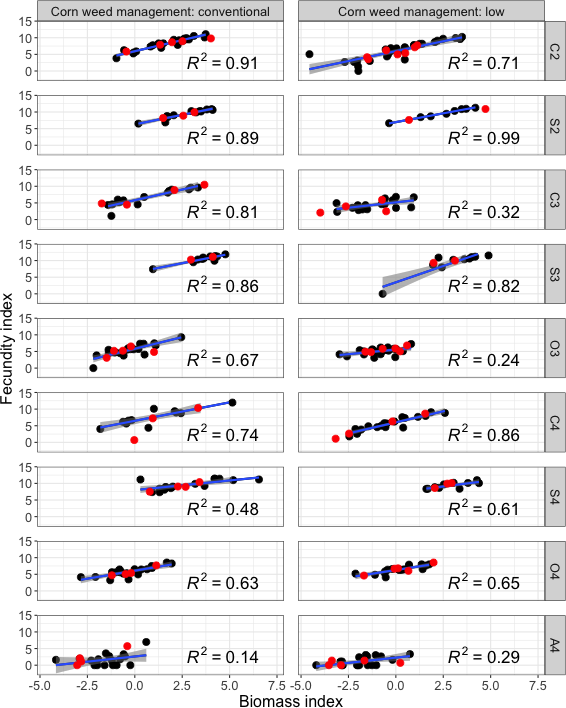
\includegraphics[width=1\linewidth]{Manuscript_whole_files/figure-latex/full-p-1} \caption{The black and red dots are values from training and testing sets, respectively. Each regression line was plotted for one crop identity by herbicide treatment using the training set. Biomass index = ln(gram biomass + 0.005) and Fecundity index = ln(seeds + 1)}\label{fig:full-p}
\end{figure}

\hypertarget{population-aboveground-mass-and-stand-density}{%
\subsection*{Population aboveground mass and stand density}\label{population-aboveground-mass-and-stand-density}}
\addcontentsline{toc}{subsection}{Population aboveground mass and stand density}

In both years, population aboveground mass and stand density was strongly influenced by crop identity (Table \ref{tab:pop-biom-dens-jt}). The rotation system in which a crop was grown also affected population aboveground mass and stand density, although not consistently between years (Table \ref{tab:pbiom-dens-ct}).

In 2018, population aboveground mass in the same crop species was comparable across rotations except for corn grown in the 2-year (C2) versus 4-year rotation (C4) (p-value = 0.043). In 2019, population aboveground mass in the same crop was significantly different across rotations, except for corn in the 2-year (C2) versus 3-year rotation (C3) (p-value = 0.968) and soybean in the 3-year (S3) versus 4-year rotation (S4) (p-value = 1). Averaged across rotations, population aboveground mass was comparable in 2018 for corn versus alfalfa (p-value = 0.2509) and soybean versus oat (p-value = 0.504), but 10- to 2580-fold different in the other ten pairs (p-values \textless{} 0.01).

In 2018, population stand density in the same crop species was comparable across the rotations. In 2019, population stand density in the same crop species was comparable for soybean (p-values = 0.1256 and 1) and C2 versus C3 (p-value = 0.9284), but significantly different for the other corn comparisons and for oat in the 3-year (O3) versus 4-year rotation (O4). Averaged over rotations, population stand density was comparable in 2018 between soybean and alfalfa (p-value = 0.766), but 5- to 1330-fold different in the other eight pairs of comparison (p-values \textless{} 0.001).

In 2018, population aboveground mass was the highest in soybean and oat (Figure \ref{fig:pop-biom-dens-all}A) because soybean weed management was ineffective and herbicide was intentionally not applied in oat. The legacy of an ineffective weed management program in 2018 soybean plots was observed in 2019 oat plots where population aboveground mass and stand density were the highest among all the crop identities ((Figure \ref{fig:pop-biom-dens-all}B). High stand density in 2019 oat plots was also due to uneven oat establishment. The change in 2019 in weed management for soybean substantially reduced the waterhemp pressure on soybean (Figure \ref{fig:pop-biom-dens-all}B and \ref{fig:pop-biom-dens-all}D).

\begin{landscape}\begin{table}

\caption{\label{tab:pop-biom-dens-jt}ANOVAs of crop identity and corn weed management effects on waterhemp population aboveground mass and stand density. Crop identity was the only influential factor on both population aboveground mass and stand density in 2018 and 2019.}
\centering
\begin{tabular}[t]{llllll>{}l|llll}
\toprule
\multicolumn{3}{c}{ } & \multicolumn{4}{c}{2018} & \multicolumn{4}{c}{2019} \\
\cmidrule(l{3pt}r{3pt}){4-7} \cmidrule(l{3pt}r{3pt}){8-11}
\multicolumn{3}{c}{ } & \multicolumn{2}{c}{\makecell[c]{Population \\ aboveground mass}} & \multicolumn{2}{c}{\makecell[c]{Population \\ stand density}} & \multicolumn{2}{c}{\makecell[c]{Population \\ aboveground mass}} & \multicolumn{2}{c}{\makecell[c]{Population \\ stand density}} \\
\cmidrule(l{3pt}r{3pt}){4-5} \cmidrule(l{3pt}r{3pt}){6-7} \cmidrule(l{3pt}r{3pt}){8-9} \cmidrule(l{3pt}r{3pt}){10-11}
Source of variation & df1 & df2 & F.value & p.value & F.value & p.value & F.value & p.value & F.value & p.value\\
\midrule
Crop ID & 8 & 51 & 21.227 & <.0001 & 27.447 & <.0001 & 42.141 & <.0001 & 84.032 & <.0001\\
Corn weed management & 1 & 51 & 0.411 & 0.5241 & 0.869 & 0.3555 & 1.228 & 0.2730 & 0.296 & 0.5889\\
Crop ID x Corn weed management & 8 & 51 & 0.403 & 0.9139 & 0.965 & 0.4736 & 1.349 & 0.2415 & 0.630 & 0.7486\\
\bottomrule
\end{tabular}
\end{table}
\end{landscape}

\textbackslash begin\{figure\}{[}H{]}
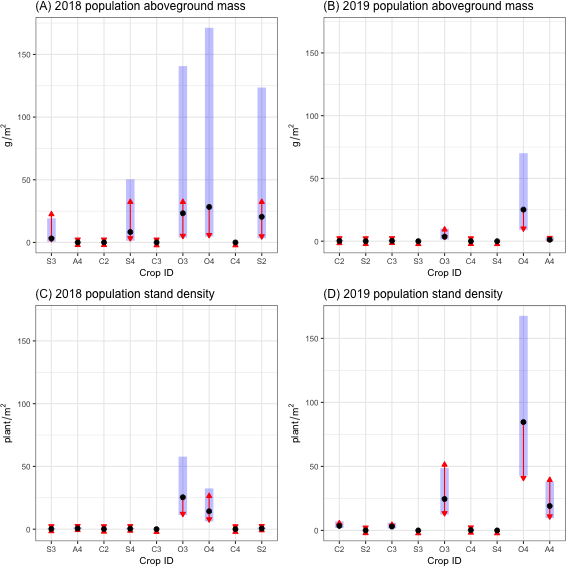
\includegraphics[width=1\linewidth]{Manuscript_whole_files/figure-latex/pop-biom-dens-all-1} \textbackslash caption\{Waterhemp population aboveground mass and stand density averaged over corn weed managements. The black dots are estimated marginal means. The blue bars are 95\% confidence intervals. The red arrows reflect the comparison among means. Overlapping arrows indicate non-significant differences.\}\label{fig:pop-biom-dens-all}
\textbackslash end\{figure\}

\begin{table}

\caption{\label{tab:pbiom-dens-ct}Rotation system and crop effects on population aboveground mass and stand density.}
\centering
\begin{threeparttable}
\begin{tabular}[t]{lrlr>{}l|rlrl}
\toprule
\multicolumn{1}{c}{ } & \multicolumn{4}{c}{2018} & \multicolumn{4}{c}{2019} \\
\cmidrule(l{3pt}r{3pt}){2-5} \cmidrule(l{3pt}r{3pt}){6-9}
\multicolumn{1}{c}{ } & \multicolumn{2}{c}{\makecell[c]{Population \\ aboveground mass}} & \multicolumn{2}{c}{\makecell[c]{Population \\ stand density}} & \multicolumn{2}{c}{\makecell[c]{Population \\ aboveground mass}} & \multicolumn{2}{c}{\makecell[c]{Population \\ stand density}} \\
\cmidrule(l{3pt}r{3pt}){2-3} \cmidrule(l{3pt}r{3pt}){4-5} \cmidrule(l{3pt}r{3pt}){6-7} \cmidrule(l{3pt}r{3pt}){8-9}
Contrast & ratio & p.value & ratio & p.value & ratio & p.value & ratio & p.value\\
\midrule
\addlinespace[0.3em]
\multicolumn{9}{l}{\textbf{(A) - Crop phase effects}}\\
\hspace{1em}C2 vs C3 & 12.54 & 0.1237 & 2.38 & 0.2990 & 0.84 & 0.9680 & 1.19 & 0.9284\\
\hspace{1em}C2 vs C4 & 23.12 & 0.0430 & 1.84 & 0.5435 & 10.61 & 0.0054 & 14.45 & <.0001\\
\hspace{1em}C3 vs C4 & 1.84 & 0.8798 & 0.78 & 0.8983 & 12.65 & 0.0026 & 12.11 & <.0001\\
\hspace{1em}S2 vs S3 & 6.42 & 0.3151 & 2.07 & 0.4258 & 6.27 & 0.0369 & 2.60 & 0.1265\\
\hspace{1em}S2 vs S4 & 2.45 & 0.7597 & 1.29 & 0.8976 & 6.27 & 0.0369 & 2.60 & 0.1265\\
\hspace{1em}S3 vs S4 & 0.38 & 0.7298 & 0.62 & 0.6963 & 1.00 & 1.0000 & 1.00 & 1.0000\\
\hspace{1em}O3 vs O4 & 0.82 & 0.8774 & 1.78 & 0.3235 & 0.14 & 0.0096 & 0.29 & 0.0132\\
\addlinespace[0.3em]
\multicolumn{9}{l}{\textbf{(B) - Crop species effects}}\\
\hspace{1em}oat vs soybean & 0.00 & <.0001 & 0.04 & <.0001 & 2580.38 & <.0001 & 1327.35 & <.0001\\
\hspace{1em}oat vs corn & 0.00 & <.0001 & 0.07 & <.0001 & 85.31 & <.0001 & 32.61 & <.0001\\
\hspace{1em}oat vs alfalfa & 0.00 & <.0001 & 0.12 & 0.0005 & 8.34 & 0.0071 & 2.39 & 0.1712\\
\hspace{1em}soybean vs corn & 1.50 & 0.9458 & 1.60 & 0.4978 & 0.03 & <.0001 & 0.03 & <.0001\\
\hspace{1em}soybean vs alfalfa & 0.09 & 0.1172 & 2.82 & 0.1366 & 0.00 & <.0001 & 0.00 & <.0001\\
\hspace{1em}corn vs alfalfa & 0.06 & 0.0488 & 1.76 & 0.6279 & 0.10 & 0.0014 & 0.07 & <.0001\\
\bottomrule
\end{tabular}
\begin{tablenotes}[para]
\item \textit{Note: } 
\item Some zero values are due to rounding.
\end{tablenotes}
\end{threeparttable}
\end{table}

\hypertarget{population-sex-ratio-1}{%
\subsection*{Population sex ratio}\label{population-sex-ratio-1}}
\addcontentsline{toc}{subsection}{Population sex ratio}

Population stand density was included to improve the precision of estimates of population sex ratios (Table \ref{tab:sexr18-covar-jt}C versus \ref{tab:sexr18-covar-jt}A). The population sex ratio in 2018 differed significantly among treatments, at different population stand densities within each treatment (p-value = 0.0155, Table \ref{tab:sexr18-covar-jt} and Figure \ref{fig:sexr18-dens-arrow}). Therefore, sex ratios in the same treatment were evaluated at four population densities, i.e., 1, 5, 50, and 500 plants/m\(^2\), to illustrate that three-way interaction (Figure \ref{fig:sexr18-dens-arrow}). Female-biasedness was more likely if a waterhemp population was grown in oat and alfalfa. None of the waterhemp populations grown in corn and soybean expressed gender biasedness. It is unclear whether the corn weed management program had a significant effect on gender biasedness given the magnitude of the variance (Figure \ref{fig:sexr18-dens-arrow}).

We defined a useful imputed data set to be a set that resulted in fully estimable marginal means for sex ratio comparison across all treatments, which was achievable with non-zeros in female and male categories in at least one replication among the four blocks for the missing observations in the 2019 original sex data. Unlike the 2018 data, the sex ratio in 2019 was analyzed without the covariates because none of the covariates improved the goodness of fit for the analysis model. With m = 24, five imputed data sets were useful (Appendix B). The significance and influence of treatment factors and their interaction in the imputed data sets for waterhemp sex ratio in 2019 were consistent with those of the 2018 data (Figure \ref{fig:sexr19-arrow}). In 21 out of 24 sets, sex ratio in 2019 was affected by crop identity (Figure \ref{fig:sexr19-arrow}B and \ref{fig:sexr19-arrow}C). Female biasedness was observed in oat and alfalfa but not in corn and soybean (Figure \ref{fig:sexr19-arrow}A).

\begin{landscape}\begin{table}

\caption{\label{tab:sexr18-covar-jt}ANOVAs of crop identity, herbicide, and covariate effects on population sex ratio using 2018 data. With population aboveground mass covariate included (B), crop identity was the only influential factor on population sex ratio. With population stand density covariate included (C), sex ratio responded differently in each treatment and stand density combination.}
\centering
\resizebox{\linewidth}{!}{
\begin{tabular}[t]{lllrl}
\toprule
Source of variation & df1 & df2 & F.ratio & p.value\\
\midrule
\addlinespace[0.3em]
\multicolumn{5}{l}{\textbf{(A) no covariate. Residual deviance = 165.9, dispersion = 3.32.}}\\
\hspace{1em}Crop ID & 8 & Inf & 8.5 & <.0001\\
\hspace{1em}Corn weed management & 1 & Inf & 0.0 & 0.9317\\
\hspace{1em}Crop ID x Corn weed management & 8 & Inf & 0.5 & 0.8862\\
\addlinespace[0.3em]
\multicolumn{5}{l}{\textbf{(B) with population aboveground mass covariate. Residual deviance = 104.3, dispersion = 3.24.}}\\
\hspace{1em}Crop ID & 8 & Inf & 1.0 & 0.4155\\
\hspace{1em}Corn weed management & 1 & Inf & 0.0 & 0.9601\\
\hspace{1em}Population aboveground mass & 1 & Inf & 1.5 & 0.2198\\
\hspace{1em}Crop ID x Corn weed management & 8 & Inf & 0.7 & 0.6847\\
\hspace{1em}Crop ID x Population aboveground mass & 8 & Inf & 1.0 & 0.4038\\
\hspace{1em}Corn weed management x Population aboveground mass & 1 & Inf & 2.8 & 0.0916\\
\hspace{1em}Crop ID x Corn weed management x Population aboveground mass & 8 & Inf & 1.2 & 0.2713\\
\addlinespace[0.3em]
\multicolumn{5}{l}{\textbf{(C) with population stand density covariate. Residual deviance = 82.12, dispersion = 2.54.}}\\
\hspace{1em}Crop ID & 8 & Inf & 1.0 & 0.4679\\
\hspace{1em}Corn weed management & 1 & Inf & 0.9 & 0.3346\\
\hspace{1em}Population stand density & 1 & Inf & 2.5 & 0.1169\\
\hspace{1em}Crop ID x Corn weed management & 8 & Inf & 1.5 & 0.1675\\
\hspace{1em}Crop ID x Population stand density & 8 & Inf & 1.7 & 0.0896\\
\hspace{1em}Corn weed management x Population stand density & 1 & Inf & 5.2 & 0.0231\\
\hspace{1em}Crop ID x Corn weed management x Population stand density & 8 & Inf & 2.4 & 0.0155\\
\bottomrule
\end{tabular}}
\end{table}
\end{landscape}

\textbackslash begin\{figure\}{[}H{]}
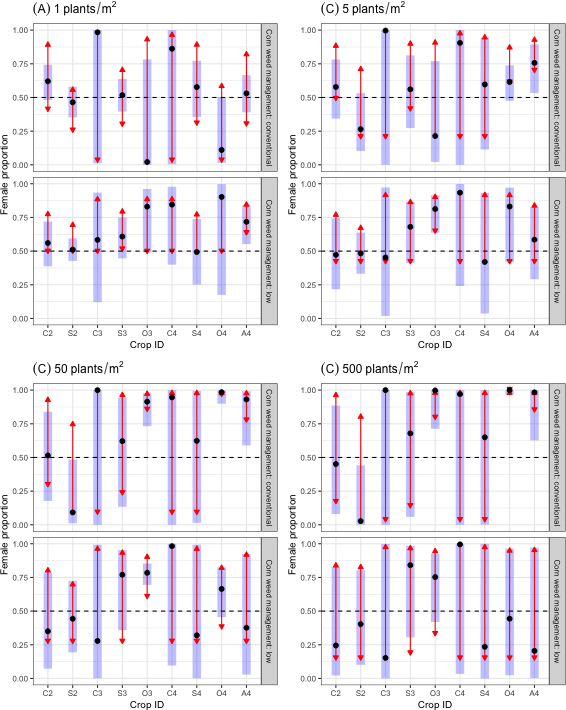
\includegraphics[width=1\linewidth]{Manuscript_whole_files/figure-latex/sexr18-dens-arrow-1} \textbackslash caption\{Waterhemp population sex ratios under 54 combinations of experimental treatments and population stand densities. The dashed lines mark sex ratio parity. The black dots are estimated marginal means. The blue bars are 95\% confidence intervals. The red arrows reflect the comparisons among means. Overlapping arrows indicate non-significant differences.\}\label{fig:sexr18-dens-arrow}
\textbackslash end\{figure\}

\begin{figure}[H]
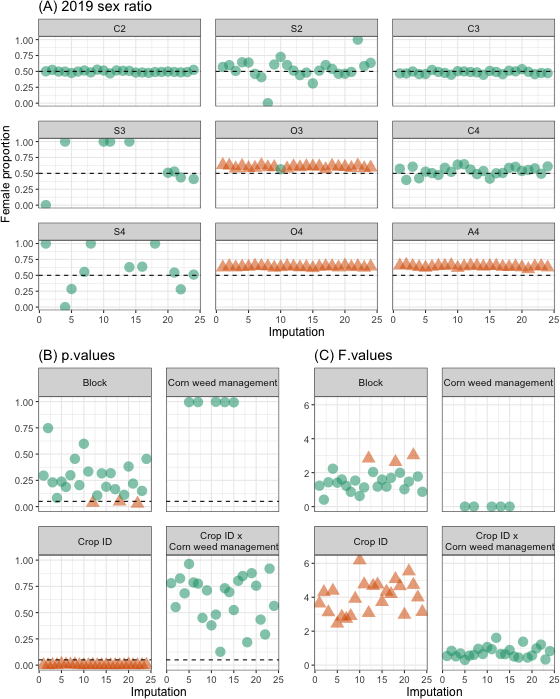
\includegraphics[width=1\linewidth]{Manuscript_whole_files/figure-latex/sexr19-arrow-1} \caption{Waterhemp population sex ratios under nine crop idenitites averaged over two Corn weed management regimes using 2019's 24 imputed data sets (A). The dashed lines mark sex ratio parity in panel A and level of confidence in panel B, respectively. The blank spaces are nonestimable values. The triangulars and circles in panel A represent female-biased and even populations assessed at alpha = 0.05, respectively. F-ratios for sources of variation are shown in panel C.}\label{fig:sexr19-arrow}
\end{figure}

\hypertarget{discussion}{%
\section*{Discussion}\label{discussion}}
\addcontentsline{toc}{section}{Discussion}

Results of this study indicate that waterhemp was affected by crops and crop management in multiple ways, including a reduction in individual biomass and fecundity to the point of non-existence as occurred in 2019 soybean plots.
Despite the 2018 and 2019 data being overdispersed, which resulted in high residual deviance, the significance of treatment effects was consistent. Crop identity was the most influential factor for all responses. Some covariation relationships were observed: population stand density affected sex ratio and female aboveground mass was a reliable predictor for fecundity.

Waterhemp is a small-seeded species that is more sensitive to environmental stress than larger-seeded species \citep{harburLightGrowthRate2004}. In the present study, the number of stress and mortality factors likely increased as crop diversity increased temporally and spatially \citep{martinEffectCropRotation1993}. Stress and mortality factors arose from the strategic cropping system designs that employ crops of different phenology, management requirements, and relative competitiveness with weeds \citep{liebmanSustainableWeedManagement1990, liebmanCropRotationIntercropping1993}.

The two summer annual row crops in our study, corn and soybean, differed from the cool season and perennial crops, oat, red clover, and alfalfa with regard to the strongest selection pressure against weeds: herbicides. In corn (C2, C3, and C4), weeds were controlled with broadcast herbicide (conventional), or a combination of banded herbicide (38-cm strips on top of crop rows) and interrow cultivation. In soybean (S2, S3, and S4), weeds were controlled with broadcast herbicide as in conventional corn, with different active ingredients. In contrast, in the O3, O4, and A4 treatments, no herbicide or cultivation was applied, but those three crops were strategically introduced to the 3-year and 4-year rotations for their potential allelopathic and shading effects \citep{liebmanCropRotationIntercropping1993, singhAllelopathicInteractionsAllelochemicals2003}. The spring establishment of O3 and O4 and overwintering of A4 treatments gave the crops a headstart for resource competition against waterhemp, a summer annual weed that emerged later \citep{hartzlerEffectCommonWaterhemp2004}. The timing of oat harvest in late July matched waterhemp's early reproductive stage \citep{buhlerRelativeEmergenceSequence2008, horakGrowthAnalysisFour2000} and the resulting mechanical damage at this stage reduced the weed's reproductive potential. Intercropping oat and alfalfa can produce stronger weed suppression than might be achieved by each species grown as a sole crop \citep{laniniFightWeedsIncrease1992}, whereas the effects of intercropping oat with red clover can be more variable \citep{samsonChoiceManagementCover1990}. For established alfalfa in the 4-year rotation, three to four hay cuts per crop season also served as a significant means of physical control and to reduce waterhemp reproductive potential.

High waterhemp population stand densities in oat resulted from highly productive plants in the preceding corn and soybean phases of the rotation and signaled abundant replenishment of soil seedbanks. \citet{dykeSuppressionCouchGrass1976} found that a clover and cereal intercrop substantially reduced weed emergence whereas \citet{heggenstallerSeasonalPatternsPostdispersal2006} found that a triticale (\emph{x Triticosecale} Wittmack) and red clover intercrop increased weed seedling recruitment. Taking these findings with the present study's observation that higher waterhemp population stand densities and lower waterhemp aboveground mass were found in small grain and forage crops than in row crops, it is possible that cold-tolerant crops can be used to stimulate and induce fatal germination to deplete the soil seedbank \citep{davisCroppingSystemEffects2003, gallandtEffectCovercroppingSystems2005}. Eventually, as more mortality and stress factors are imposed on emerged weeds via various control methods, such as allelopathy and mechanical damage via crop harvest, those emerged plants might be expected to contribute fewer seeds to the soil seedbank.

Waterhemp populations in three of the treatments, O3, O4, and A4, were slightly female-biased. Waterhemp populations in other treatments were even in sex ratio, which might be attributed to a more stressful conditions in small grain and forage crops than in row crops. A larger data set might help reducing the variance in sex ratio and provide a clearer understanding of the effect of corn weed management program on waterhemp sex ratio in subsequent oat and alfalfa phases. Systematic analysis is needed to identify the contribution of each stressor on waterhemp development and population dynamics. The 2019 sex ratio data were imputed without 2018 input but returned consistent conclusions on treatment effects, as compared to 2018. This consistency suggests an acceptable precision of the analysis model and the imputation algorithm. Since \texttt{pmm} seeks to fill in missing values with placeholders without changing the overall mean, it is reasonable to assume that the sex ratios in soybean eu's were even. The high herbicide efficacy in soybean was the strongest selection pressure on the exposed waterhemp populations.

Our analysis indicated that female aboveground mass could be used to predict fecundity parsimoniously. The strong evidence of the significant interaction effect of weed management regime and crop identity on waterhemp fecundity justified the use of separate equations for each treatment. Since different sources of stress were introduced in the small grain and forages than in row crops, we attributed female-biasedness and lower fecundity in forages than in row crops to female herbaceous plants outperforming males under abiotic and biotic stresses \citep{juvanySexrelatedDifferencesStress2015}. The stand density and sex ratio data in this study does not provide sufficient information to establish a relationship between them, as was established between individual female biomass and fecundity. It would be helpful to explore the population stand density and sex ratio relationship with a bigger data set.

In the present study, using mother plant reproduction potential (aboveground mass) gives a rough estimate of the number of seeds being added to the soil seedbank. Additionally, the total number of seeds produced at the end of the season in each treatment depended on the parent plant density and population sex ratio. The possibility of post-harvest seed loss due to seed predators under different ground cover conditions adds to the complexity of seedbank dynamics. Red clover that remained after oat harvest and alfalfa living mulch may enhance granivore activities \citep{davisCroppingSystemEffects2003, gallandtEffectCovercroppingSystems2005}. \citet{heggenstallerSeasonalPatternsPostdispersal2006} found increased predation of velvetleaf (\emph{Abutilon theophrasti} Medik) and giant foxtail (\emph{Setaria faberi} Herrm) seeds in more diverse cropping systems than in shorter corn-soybean rotations. Overwintering crops such as alfalfa delayed pigweed (\emph{Amaranthus quitensis} H.B.K.) emergence \citep{huarteUnderstandingMechanismsReduced2003} and can exude allelochemicals for weed suppression \citep{millerAllelopathyForageCrop1996}. Compared to the bare ground after corn and soybean production, the post-harvest environment in oat and alfalfa may induce more seed loss due to predation \citep{gallandtEffectCovercroppingSystems2005}. Waterhemp was not included in the \citet{heggenstallerSeasonalPatternsPostdispersal2006} study, but waterhemp seeds are preferred over other species' seeds by field crickets and ground beetles \citep{vanderlaatPostdispersalWeedSeed2015} so it is likely that the small gran and forage crops in the present study enhanced waterhemp seed predation.

More investigation is needed to determine how soil seedbank dynamics contribute to population dynamics in different scenarios, such as how female-biasedness could be potentially helpful to replenish a seedbank, whether sexual unevenness in a generation causes sexual unevenness in freshly produced seeds, and how those biases contribute to long-term population changes and competitiveness against crops. In the near-total control situation as occurred in the 2019 soybean plots, as the number of fresh seeds added to the soil seedbank can be considered negligible, other factors, such as sex ratio, population stand density, and plant size are of less practical concern. A more practical investigation would be to see how different levels of control efficacy translate into medium- and long-term population changes, because no herbicide is totally invulnerable to the evolution of resistance in weed populations. It would also be useful to see how populations would change once resistance occurred and how various control methods might contribute to resistance management.

\hypertarget{appendix}{%
\section*{Appendix}\label{appendix}}
\addcontentsline{toc}{section}{Appendix}

\hypertarget{appendix-a}{%
\subsection{Appendix A}\label{appendix-a}}

\emph{Seed cleaning and counting procedure}

The following protocol was used to separate seeds from stems and to clean seeds.

Step 1 - A whole sample was run through a brushing machine (LA-H, Westrup, Slageise, Denmark) to break the fruits from the stem. Large samples were chopped before running through the machine.

Step 2 - Chaff-covered seeds were run through a stack of two sieves (U.S. Standard Sieve Series), one that was 710 micron on top and one that was 297 micron at the bottom in a shaker (Dayton, Seedburo Equipment Company). The sieve stack was securely closed with a top and a bottom lid. The 297-micron sieve was used to separate small stems, while the 710-micron sieve separated the dust from the seeds. Seeds at this step were still chaffy and partially enclosed in the fruits. Seeds that were still enclosed at this step did not pass the top sieve and were rubbed with rubber bands (Step 4). Small pieces of stems and dust were discarded. The material in between the two sieves was retained.

Step 3 - The material between the two sieves from step 2 was run through a custom-made dual-slope separator (Iowa State University Seed Laboratory) to separate clean seeds and chaffed seeds.

Step 4 - The pericarps from step 3 were rubbed in between rubber bands to remove capsules.

Step 5 - Seeds from steps 3 and 4 were run separately through a blower (CB-1, Agriculex Inc, Guelph, Canada) to remove the remaining capsules. The blower was started at the lowest wind speed and adjusted throughout the blowing process so that as much of the chaff and foreign materials were removed as possible while seeds were retained.

Step 6 - Steps 3 to 5 were repeated depending on the cleanliness of the material.

Step 7 - Cleaned seeds were enumerated with either an Old Mill Counter (850-3, International Marketing and Design Corp) or a Ball Coleman optical counter (Gen3, Ball Horticultural Company, Illinois, USA). The Ball Coleman optical counter was with a precision of 0.16\% difference between samples several times per sample. With Old Mill Counter, seeds were counted once. With the Old Mill Counter or by hand, each sample were counted once. With the Ball Coleman optical counter, each samples were counted several times and three counts that were the least different from one another were averaged and used as the sample's seed count.

\emph{Seed sample preparation and machine calibration}

Seeds to be counted were threshed by hand or machine, depending on plant size, and then cleaned of chaff.
Samples of hundreds of seeds were counted by hand, larger samples with either an Old Mill Counter or a Ball Coleman optical Counter. Before counting, each sample bag was weighed, i.e., bag, tag, and plant material, then the bag and tag.
Plant weight was obtained by subtracting the bag and tag weight from the sample bag weight.
Seeds must be fairly clean in order to be counted with machines.
Obtaining clean seed samples without chaff and foreign materials was extremely time-consuming, so we trained an optical counter to eliminate particles whose sizes were noticeably different from the mean seed size of roughly 1 mm diameter \citep{bellTimeRequirementPollination2010}.
The Ball Coleman optical counter was calibrated to count waterhemp seeds by running a ``known sample'' of 1200 seeds (a sample that was counted by hand) to establish a learning function to eliminate particles that were very much smaller and larger than the mean seed size from the final count.
The ``known sample'' was run through the optical counter at 2300 seeds/second, uncalibrated, to obtain a distribution of all the counted particles.
The counting rate of 2300 seeds/second was automated by the counter after running a small batch of seeds in such a way that a steady, single-file seed flow was maintained during the counting process.
Two tails of the distribution of particle sizes, i.e., too large and too small, were trimmed in such a way that the new counts were closest to the hand-counted number.
In our case, any counted particles whose surface area was larger than 0.1963 mm\(^2\) were removed from the total count in the learning function.
Once the learning function was established, seeds were counted with reference to the saved settings.
The known sample was recounted with the calibrated counter to confirm the result.

\hypertarget{appendix-b-2019-sex-ratio-imputation}{%
\subsection*{Appendix B: 2019 sex ratio imputation}\label{appendix-b-2019-sex-ratio-imputation}}
\addcontentsline{toc}{subsection}{Appendix B: 2019 sex ratio imputation}

\hypertarget{data-set-and-imputation-procedure-overview}{%
\subsubsection*{Data set and imputation procedure overview}\label{data-set-and-imputation-procedure-overview}}
\addcontentsline{toc}{subsubsection}{Data set and imputation procedure overview}

The experiment design was RCBD with four blocks, nine levels of main plot (Crop ID) and two levels of split-plot (Corn weed management) effects. There were 72 experiment units (eu), 8 observational units (quadrats) per eu. Within each quadrats, six cohorts of plants were sexed. By the time that the plants were sexed, a few plants' sexes were not observable and thus, they are marked as Unknown in the data set. This caused Total \textgreater{} Male + Female in some eu's.

Complete case analysis, in which missing observations are removed from the data set, is acceptable when less than 5\% of the data is missing at random because removing the incomplete cases does not significantly change the outcome \citep{azurMultipleImputationChained2011}. The 2019 sex ratio is imputed because 22\% of the data (755 \texttt{NA}s out of 3448 entries) was missing at random (MAR). We considered our data MAR even though the number of missing values were higher in soybean plots than in the other three crops because 1) the quadrats were placed randomly in the field before weed emergence, 2) waterhemp and other weed seedlings were present in the quadrats at the beginning of the season, and 3) waterhemp and other weed species were found in soybean plots by the time we sexed the waterhemp plants, but not in the eight fixed quadrats.

The MICE imputation method assumes that after controlling for all the observation in the original data set, all the missingness occurs at random \citep{vanbuurenMiceMultivariateImputation2011}. A good imputation model is numerically recognized by low fraction of information missing due to nonresponse (\texttt{fmi}), small proportion of total variance that is attributable to the missing data (\(\lambda\)) values; and visually recognized by the similarity in kernel density estimates and data points distribution between the observed and imputed data sets \citep{vanbuurenMiceMultivariateImputation2011}. The number of imputations (m) should be chosen such that the loss of efficiency, \(le = \frac{fmi}{m} \leq 0.05\) \citep{whiteMultipleImputationUsing2011}. To give the imputation model more information, the data was imputed using 3448 data points. The analysis model on the imputed data sets was run using 72 data points.

The recommended specifications of the imputation model for this data set are: 1) uses at least 24 imputations (24 was selected because it is divisible by 4 cores in the computer processor), 2) includes all the covariates (Number of emerged seedlings, Male, Female, and Total) and predictors in the analysis model, and 3) uses an overdispersed Poisson regression model \citetext{\citealp{azurMultipleImputationChained2011}; \citealp{whiteMultipleImputationUsing2011}; \citealp[and][]{nguyenModelCheckingMultiple2017}}. While the first two specifications were met, overdispersed Poisson regression model could not be specified. The extensions for count data mentioned in Chapter 7 \citep{vanbuurenFlexibleImputationMissing2018} do not fit this data set well. Both \texttt{micemd}'s \texttt{mice.impute.2l.glm.pois} and \texttt{mice.impute.2l.2stage.pois} functions impute the numbers of Male, Female, and Total separately \citep{audigierMicemdMultipleImputation2019}. The predictive mean matching (\texttt{pmm}) method in the \texttt{mice} package can handle counts \citep{vanbuurenMiceMultivariateImputation2011} and is the optimal solution for this data set at this writing (Figure \ref{fig:kernel-xy-imp1-all-diag}).

\hypertarget{diagnosis-of-the-imputation-model-with-m-24}{%
\subsubsection*{Diagnosis of the imputation model with m = 24}\label{diagnosis-of-the-imputation-model-with-m-24}}
\addcontentsline{toc}{subsubsection}{Diagnosis of the imputation model with m = 24}

The imputation code with predicted mean matching (\texttt{pmm}) method is provided in the Supplementary Material section. Each round of imputation is distinguished by the number of imputation (m). The loss of efficiency (le) are all below the recommended value of 0.05 \citep{whiteMultipleImputationUsing2011} for the analysis model terms using the imputed data sets, under three m values and the imputation performance improved as m increased (Table \ref{tab:pool-diag}). m was capped at 2400 imputations for this manuscript because of limited computational power.\\
The diagnosis of data imputation is demonstrated here with m = 24 for ease of view. The distribution of the imputed data sets match that of the observation (Figure \ref{fig:kernel-xy-imp1-all-diag}) so the outputs (imputed data sets) were used for further regression analyses that involved sex ratio.

\hypertarget{diagnosis-of-the-analysis-model-with-m-24}{%
\subsubsection*{Diagnosis of the analysis model with m = 24}\label{diagnosis-of-the-analysis-model-with-m-24}}
\addcontentsline{toc}{subsubsection}{Diagnosis of the analysis model with m = 24}

The similarity in the magnitude of reduction of deviance and dispersion values suggests comparable, small impacts of population aboveground mass and population stand density covariates on the improvement of the goodness of fit for comparing sex ratio using 2019 imputed data (Data Repository). In addition, using either of them as a covariate in the analysis models resulted in nonestimable corn weed management effects on sex ratios in some treatments, so 2019 sex ratios were averaged over corn weed management regimes and compared without any covariates for simplicity.

\begin{figure}[H]
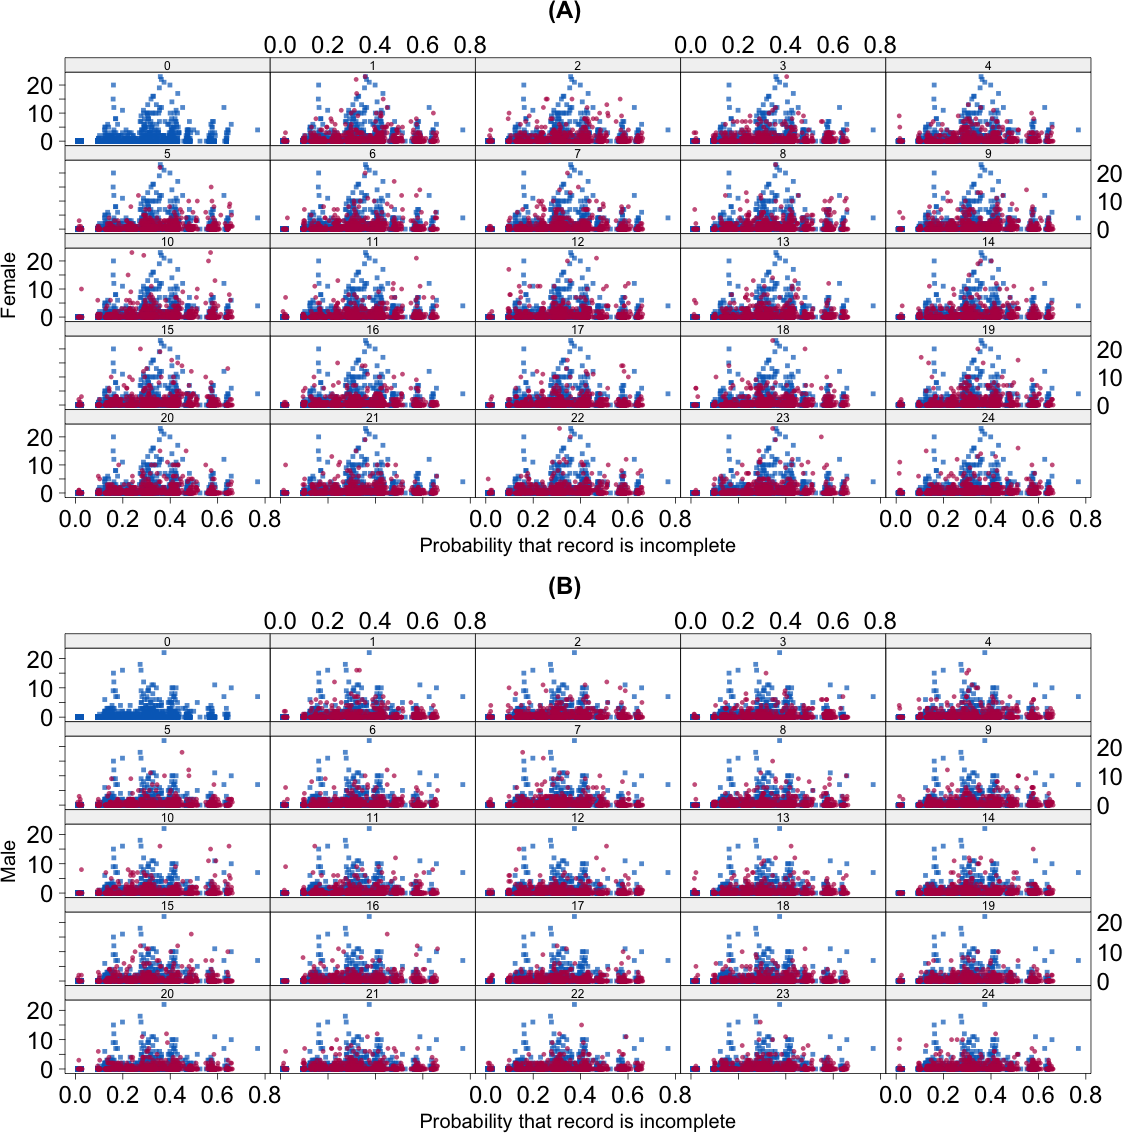
\includegraphics[width=1\linewidth]{Manuscript_whole_files/figure-latex/kernel-xy-imp1-all-diag-1} \caption{Number of female (A) and male (B) against the missingness probability for observed (data set numbered 0) and imputed data (data set numbered 1 to 24).}\label{fig:kernel-xy-imp1-all-diag}
\end{figure}

\begin{landscape}\begin{table}

\caption{\label{tab:pool-diag}Imputation model indices with different values of m. NAs resulted from nonestimable number of male and female in a treatment.}
\centering
\resizebox{\linewidth}{!}{
\begin{tabular}[t]{lrr>{}rrr>{}rrr>{}rrr>{}rrr>{}r}
\toprule
\multicolumn{1}{c}{ } & \multicolumn{3}{c}{n/m} & \multicolumn{3}{c}{riv} & \multicolumn{3}{c}{fmi} & \multicolumn{3}{c}{lambda} & \multicolumn{3}{c}{le} \\
\cmidrule(l{3pt}r{3pt}){2-4} \cmidrule(l{3pt}r{3pt}){5-7} \cmidrule(l{3pt}r{3pt}){8-10} \cmidrule(l{3pt}r{3pt}){11-13} \cmidrule(l{3pt}r{3pt}){14-16}
term & m = 24 & m = 240 & m = 2400 & m = 24 & m = 240 & m = 2400 & m = 24 & m = 240 & m = 2400 & m = 24 & m = 240 & m = 2400 & m = 24 & m = 240 & m = 2400\\
\midrule
(Intercept) & 0.2083 & 0.1167 & 0.1433 & 0.3739 & 0.3644 & 0.3386 & 0.2793 & 0.2699 & 0.2554 & 0.2722 & 0.2671 & 0.2529 & 0.0116 & 0.0011 & 0.0001\\
Block: 2 & 0.2083 & 0.1167 & 0.1433 & 0.5344 & 0.5998 & 0.5840 & 0.3575 & 0.3781 & 0.3712 & 0.3483 & 0.3749 & 0.3687 & 0.0149 & 0.0016 & 0.0002\\
Block: 3 & 0.2083 & 0.1167 & 0.1433 & 0.5804 & 0.5371 & 0.5117 & 0.3770 & 0.3525 & 0.3410 & 0.3672 & 0.3494 & 0.3385 & 0.0157 & 0.0015 & 0.0001\\
Block: 4 & 0.2083 & 0.1167 & 0.1433 & 0.9424 & 0.7040 & 0.6527 & 0.4978 & 0.4164 & 0.3975 & 0.4852 & 0.4131 & 0.3949 & 0.0207 & 0.0017 & 0.0002\\
Crop ID: C3 & 0.2083 & 0.1167 & 0.1433 & 0.3516 & 0.4493 & 0.4273 & 0.2669 & 0.3130 & 0.3019 & 0.2601 & 0.3100 & 0.2994 & 0.0111 & 0.0013 & 0.0001\\
Crop ID: C2 & 0.2083 & 0.1167 & 0.1433 & 0.1682 & 0.2340 & 0.2591 & 0.1480 & 0.1923 & 0.2083 & 0.1440 & 0.1896 & 0.2058 & 0.0062 & 0.0008 & 0.0001\\
Crop ID: C4 & 0.2083 & 0.1167 & 0.1433 & 0.8327 & 0.8853 & 0.8554 & 0.4663 & 0.4730 & 0.4636 & 0.4544 & 0.4696 & 0.4610 & 0.0194 & 0.0020 & 0.0002\\
Crop ID: O3 & 0.2083 & 0.1167 & 0.1433 & 0.7229 & 0.6626 & 0.6850 & 0.4307 & 0.4018 & 0.4091 & 0.4196 & 0.3985 & 0.4065 & 0.0179 & 0.0017 & 0.0002\\
Crop ID: A4 & 0.2083 & 0.1167 & 0.1433 & 0.3330 & 0.5269 & 0.5021 & 0.2563 & 0.3482 & 0.3368 & 0.2498 & 0.3451 & 0.3343 & 0.0107 & 0.0015 & 0.0001\\
Crop ID: S2 & 0.2083 & 0.1167 & 0.1433 & 1.5154 & 0.0006 & 0.0009 & 0.6167 & 0.0031 & 0.0034 & 0.6024 & 0.0006 & 0.0009 & 0.0257 & 0.0000 & 0.0000\\
Crop ID: S3 & 0.2083 & 0.1167 & 0.1433 & NA & NA & NA & NA & NA & NA & NA & NA & NA & NA & NA & NA\\
Crop ID: S4 & 0.2083 & 0.1167 & 0.1433 & 0.0006 & NA & NA & 0.0031 & NA & NA & 0.0006 & NA & NA & 0.0001 & NA & NA\\
Corn weed managementlow & 0.2083 & 0.1167 & 0.1433 & 0.4410 & 0.4470 & 0.4214 & 0.3140 & 0.3119 & 0.2990 & 0.3060 & 0.3089 & 0.2965 & 0.0131 & 0.0013 & 0.0001\\
Crop ID: C3 x Corn weed managementlow & 0.2083 & 0.1167 & 0.1433 & 0.6788 & 0.6881 & 0.6047 & 0.4150 & 0.4109 & 0.3794 & 0.4043 & 0.4076 & 0.3768 & 0.0173 & 0.0017 & 0.0002\\
Crop ID: C2 x Corn weed managementlow & 0.2083 & 0.1167 & 0.1433 & 0.4194 & 0.8696 & 0.7311 & 0.3032 & 0.4685 & 0.4249 & 0.2955 & 0.4651 & 0.4223 & 0.0126 & 0.0020 & 0.0002\\
Crop ID: C4 x Corn weed managementlow & 0.2083 & 0.1167 & 0.1433 & 1.3038 & 1.0537 & 1.0291 & 0.5798 & 0.5166 & 0.5097 & 0.5659 & 0.5131 & 0.5072 & 0.0242 & 0.0022 & 0.0002\\
Crop ID: O3 x Corn weed managementlow & 0.2083 & 0.1167 & 0.1433 & 0.6842 & 0.6712 & 0.8059 & 0.4170 & 0.4049 & 0.4488 & 0.4062 & 0.4016 & 0.4463 & 0.0174 & 0.0017 & 0.0002\\
Crop ID: A4 x Corn weed managementlow & 0.2083 & 0.1167 & 0.1433 & 0.2450 & 0.4780 & 0.4938 & 0.2020 & 0.3264 & 0.3331 & 0.1968 & 0.3234 & 0.3306 & 0.0084 & 0.0014 & 0.0001\\
Crop ID: S2 x Corn weed managementlow & 0.2083 & 0.1167 & 0.1433 & NA & NA & NA & NA & NA & NA & NA & NA & NA & NA & NA & NA\\
Crop ID: S3 x Corn weed managementlow & 0.2083 & 0.1167 & 0.1433 & NA & NA & NA & NA & NA & NA & NA & NA & NA & NA & NA & NA\\
Crop ID: S4 x Corn weed managementlow & 0.2083 & 0.1167 & 0.1433 & NA & NA & NA & NA & NA & NA & NA & NA & NA & NA & NA & NA\\
\bottomrule
\end{tabular}}
\end{table}
\end{landscape}

\begin{landscape}\begin{table}

\caption{\label{tab:sexr19-covar-summ}Numerical diagnosis of model's goodness of fit with and without covariates on 2019 imputed data sets.}
\centering
\resizebox{\linewidth}{!}{
\begin{tabular}[t]{lllllllllllllllllllllllll}
\toprule
\addlinespace[0.3em]
\multicolumn{25}{l}{\textbf{(A) Population aboveground mass covariate}}\\
\hspace{1em}Imputation & 1 & 2 & 3 & 4 & 5 & 6 & 7 & 8 & 9 & 10 & 11 & 12 & 13 & 14 & 15 & 16 & 17 & 18 & 19 & 20 & 21 & 22 & 23 & \vphantom{2} 24\\
\hspace{1em}Deviance & 51.51 & 46.59 & 38.57 & 44.26 & 40.73 & 62.82 & 56.71 & 59.81 & 25.82 & 49.08 & 44.44 & 40.85 & 28.42 & 50.46 & 31.56 & 48.62 & 49.06 & 32.72 & 51.68 & 55.96 & 36.68 & 37.04 & 59.29 & 44.38\\
\hspace{1em}Dispersion & 2.19 & 1.99 & 1.54 & 1.74 & 1.53 & 2.42 & 2.29 & 2.49 & 1.20 & 2.02 & 1.95 & 1.71 & 1.16 & 2.11 & 1.36 & 1.96 & 1.79 & 1.29 & 2.01 & 2.38 & 1.60 & 1.43 & 2.38 & 1.73\\
\addlinespace[0.3em]
\multicolumn{25}{l}{\textbf{(B) Population stand density covariate}}\\
\hspace{1em}Imputation & 1 & 2 & 3 & 4 & 5 & 6 & 7 & 8 & 9 & 10 & 11 & 12 & 13 & 14 & 15 & 16 & 17 & 18 & 19 & 20 & 21 & 22 & 23 & \vphantom{1} 24\\
\hspace{1em}Deviance & 45.22 & 37.60 & 41.66 & 39.11 & 52.50 & 66.21 & 61.79 & 51.69 & 27.44 & 47.33 & 36.24 & 47.05 & 28.19 & 44.59 & 24.53 & 59.57 & 48.72 & 38.23 & 35.92 & 66.81 & 35.47 & 49.25 & 58.26 & 58.51\\
\hspace{1em}Dispersion & 1.98 & 1.62 & 1.67 & 1.58 & 2.00 & 2.54 & 2.55 & 2.12 & 1.28 & 1.94 & 1.59 & 1.99 & 1.16 & 1.84 & 1.05 & 2.47 & 1.79 & 1.56 & 1.40 & 2.96 & 1.54 & 1.88 & 2.41 & 2.29\\
\addlinespace[0.3em]
\multicolumn{25}{l}{\textbf{(C) No covariate}}\\
\hspace{1em}Imputation & 1 & 2 & 3 & 4 & 5 & 6 & 7 & 8 & 9 & 10 & 11 & 12 & 13 & 14 & 15 & 16 & 17 & 18 & 19 & 20 & 21 & 22 & 23 & 24\\
\hspace{1em}Deviance & 78.24 & 63.29 & 72.17 & 72.88 & 90.87 & 105.28 & 91.76 & 81.60 & 49.72 & 73.75 & 63.36 & 64.03 & 45.61 & 80.43 & 47.17 & 95.78 & 75.41 & 57.65 & 72.34 & 96.18 & 68.97 & 69.57 & 96.86 & 87.33\\
\hspace{1em}Dispersion & 2.10 & 1.72 & 1.87 & 1.82 & 2.12 & 2.56 & 2.36 & 2.07 & 1.42 & 1.99 & 1.70 & 1.71 & 1.19 & 2.03 & 1.23 & 2.42 & 1.75 & 1.48 & 1.76 & 2.52 & 1.80 & 1.66 & 2.44 & 2.15\\
\bottomrule
\end{tabular}}
\end{table}
\end{landscape}

\hypertarget{acknowledgements}{%
\section*{Acknowledgements}\label{acknowledgements}}
\addcontentsline{toc}{section}{Acknowledgements}

The authors thank Matt Woods, Mike Fiscus, and the Iowa State University's Agronomy Research Farm crew for field management; Jessica Juarez-Morales, Elizabeth Oys, Ana Poznanski, Andrew Riehl, Angela Soto-Saenz, and Wyatt Westfall for field and laboratory assistance; Alan Gaul and Iowa State University's Seed Laboratory student assistants and interns for seed cleaning laboratory space, guidance, and technical assistance; Philip Dixon and Dean Adams for data analysis assistance; Russ Lenth and other Stackoverflow community members for answering HN's coding questions; and Lisa Schulte-Moore, Micheal Owen, and Mark Gleason for reviewing the manuscript.

\renewcommand\refname{References}
  \bibliography{fecund.bib}

\end{document}
